%\PassOptionsToPackage{unicode=true}{hyperref} % options for packages loaded elsewhere
%\PassOptionsToPackage{hyphens}{url}
%
\documentclass[a4paper,12pt,openany,final]{extreport}
%\usepackage[times,fancytop,firamono,cpcaption,microtyping]{subook}
\usepackage[times,firamono,microtyping,732]{subook}
%\usepackage{booktabs}
\usepackage{multicol}
\usepackage{totcount}
\usepackage{multirow}
\usepackage{array}
\usepackage{makecell}
\usepackage{titlesec}
%\usepackage{color}
%\usepackage{soul}
\date{}
% \hypersetup{
%     bookmarks=true,         % show bookmarks bar?
%     unicode=true,           % non-Latin characters in Acrobat’s bookmarks
%     pdftoolbar=true,        % show Acrobat’s toolbar?
%     pdfmenubar=true,        % show Acrobat’s menu?
%     pdffitwindow=false,     % window fit to page when opened
%     pdfstartview={FitH},    % fits the width of the page to the window
%     pdftitle={Компьютерные науки, часть 4},    % title
%     pdfauthor={Евгений Александрович Черкашин},     % author
%     pdfsubject={Методическое пособие},   % subject of the document
%     pdfcreator={EMACS-24.4:AuCTeX},   % creator of the document
%     pdfproducer={LuaLaTeX}, % producer of the document
%     pdfkeywords={Искусственный интеллект} {Логическое
%       программирование} {Планирование действий} {Удовлетворение
%       ограничений} {Компьютерная алгебра} {Принцип максимума} {Оптимальное управление}, % list of keywords
%     pdfnewwindow=true,      % links in new window
%     colorlinks=true,       % false: boxed links; true: colored links
%     linkcolor=[rgb]{0 0.4 0.1},          % color of internal links (black)
%     citecolor=blue,        % color of links to bibliography
%     filecolor=black,      % color of file links
%     urlcolor=[rgb]{0.3 0.0 0.3}           % color of external links
%   }

% \let\oldcaption\caption
%\renewcommand{\caption}[1]{\stepcounter{lastfig}\label{LastFig}\oldcaption{#1}}
\newcommand\theyear{2017}

\usepackage{xcolor}
\usepackage{stackengine}
\setstackgap{L}{.5\baselineskip}
\newcommand\MA[2]{{\sffamily\color{red}\hsmash{$\uparrow$}%
  \smash{\toplap{#1}{\scriptsize\bfseries #2}}}}
\newcommand\MB[2]{{\sffamily\color{red}\hsmash{$\downarrow$}%
    \smash{\bottomlap{#1}{\scriptsize\bfseries#2}}}}
\usepackage{tikz}

\newcommand*{\hl}[1]{%
\tikz[baseline]\node[rectangle, fill=yellow, rounded corners, inner sep=0.3mm,anchor=base]{#1};%
}
\makeatletter
   \def\vhrulefill#1{\leavevmode\leaders\hrule\@height#1\hfill \kern\z@}
\makeatother

\newcommand\toprule{\noindent\vhrulefill{2pt}}
\newcommand\bottomrule{\noindent\vhrulefill{2pt}}
\newcommand\midrule{\noindent\vhrulefill{2pt}}

\newtotcounter{captionsnum}
\def\oldcaption{} \let\oldcaption=\caption
\def\caption{\stepcounter{captionsnum}\oldcaption}

\newtotcounter{bibitemnum}
\def\oldbibitem{} \let\oldbibitem=\bibitem
\def\bibitem{\stepcounter{bibitemnum}\oldbibitem}

\newtotcounter{appsnum}
\setcounter{appsnum}{1}

\newcommand\T{\rule{0pt}{2.6ex}}       % Top strut
\newcommand\B{\rule[-1.2ex]{0pt}{0pt}} % Bottom strut
\newcommand{\BA}[1]{%
  \begin{minipage}[b]{0.4\textwidth}
    \raggedright\T
    #1
  \end{minipage}
}
\let\BT\BA
\newcommand{\BB}[1]{%
  \begin{minipage}[t]{0.4\textwidth}
    \raggedright\T
    #1
  \end{minipage}
}
\newcommand{\BC}[2]{%
  \begin{minipage}[c]{#1}
    \raggedright\T
    #2
  \end{minipage}
}

\makeatletter
\renewcommand\bibsection{%
\chapter{\bibname}%
\@mkboth{\MakeUppercase{\bibname}}{\MakeUppercase{\bibname}}%
}%
\makeatother


\begin{document}

\clubpenalty=10000
\widowpenalty=10000

\parskip=0pt plus 0.3pt

\pagestyle{plain}
%\renewcommand{\bibname}{\appendixname~А.~Список использованных источников}
\renewcommand{\bibname}{Список использованных источников}
%\setmainfont{Calibri}
\providecommand\sfcpshape{\rmfamily}
\newcommand{\capfont}{\Large\sffamily\sfcpshape\bfseries}
\begin{titlepage}
\thispagestyle{empty}
\begin{center}

\textbf{Федеральное государственное бюджетное учреждение науки\\
Иркутский научный центр\\
Сибирского отделения Российской академии наук\\
(ИНЦ СО РАН)}

\vfill

\textbf{\large ОТЧЕТ}\\
(промежуточный)\\
за~\theyear{}~г.\\
по теме

\textbf{\large 4.1. часть 2: Применение методов NGS-BD (Next Generation Sequencing -- Big Data) для решения вопросов экологии}
\vspace{2em}

Интеграционная программа СО РАН

\textbf{Фундаментальные исследования и прорывные технологии как основа
опережающего развития Байкальского региона и его межрегиональных связей
(2017-2020 гг.)}
\vspace{1em}

Координатор программы: академик РАН И.В. Бычков
\end{center}
\vspace{1em}

\begin{tabular*}{\textwidth}{@{\extracolsep{\fill}}p{5cm}@{}p{4cm}@{}p{5cm}@{}}
Руководитель направления & & Грачёв М.А. академик, в.н.с.\\\cline{2-2}
&\vspace{0.5em}&\\
Руководители проекта & & \BT{д.б.н., проф. Лихошвай
Е.В.,\\ д.б.н. Земская Т.И.}\\\cline{2-2}
&\vspace{2em}&\\
  Исполнители проекта: & & \BB{%
ЛИН СО РАН,\\
ИДСТУ СО РАН,\\
  ИНЦ СО РАН
  }\\
\end{tabular*}

\vfill
\begin{center}
г. Иркутск,~\theyear{}~г.
\end{center}
\end{titlepage}

\begin{titlepage}
  \thispagestyle{empty}
  \begin{center}
    {\capfont РЕФЕРАТ}
  \end{center}

Отчет \pageref{LastPage}~с., \total{captionsnum}~рис., \total{bibitemnum}~источников, \total{appsnum}~прил.\\[0.2em]

Анализ больших объемов данных, информационные технологии и системы,
распределённые информационно-вычислительные ресурсы, экоинформатика,
базы данных и знаний, водные экосистемы, секвенирование нового
поколения, микробиом, корреляционные сети

\end{titlepage}
\begin{titlepage}
  \thispagestyle{empty}
  \begin{center}

    {\capfont Список основных исполнителей}
    \vspace{1em}

  {\capfont\normalsize Научные руководители части 4.1.2\\[1em]}
  \begin{tabular*}{\textwidth}{@{}l@{\hspace{3em}}@{}p{4cm}@{\extracolsep{\fill}}l@{}}
\BA{Лихошвай Е.В., д.б.н., проф.,
    зав. отд. Ультраструктуры клетки ЛИН СО РАН}&

    & Разделы~\ref{chap:1}--\ref{chap:9}\\\cline{2-2}
\BA{%
Земская Т.И., д.б.н.,
    зав. лаб. Микробиологии углеводородов ЛИН СО РАН}& & Разделы~\ref{chap:1}, \ref{chap:4}\\\cline{2-2}
    &\vspace{2em}&\\

    \multicolumn{3}{c}{
        \capfont \normalsize Основные исполнители темы
    \vspace{1em}
    }\\

\BA{Галачьянц Юрий Павлович, к.б.н., с.н.с.} & &Разделы~\ref{chap:2}, \ref{chap:3}, \ref{chap:8}\\\cline{2-2}
\BA{Петрова Дарья Петровна,\\ к.б.н., н.с.}& &                   Разделы~\ref{chap:1}, \ref{chap:3}\\\cline{2-2}
\BA{Морозов Алексей Анатольевич, гл. спец. биоинф.}& &                   Раздел~\ref{chap:6}\\\cline{2-2}
\BA{Павлова Ольга Николаевна, к.б.н., с.н.с.}& &                   Раздел~\ref{chap:4}\\\cline{2-2}
\BA{Ломакина Анна Александровна, к.б.н., с.н.с.}& &                    Раздел~\ref{chap:1}\\\cline{2-2}
\BA{Башенхаева Мария Викторовна, к.б.н., с.н.с.}& &                   Раздел~\ref{chap:3}\\\cline{2-2}
\BA{Букин Юрий Сергеевич,\\ к.б.н., с.н.с.}& &                   Разделы~\ref{chap:2}, \ref{chap:3}, \ref{chap:9}\\\cline{2-2}
\BA{Черкашин Евгений Александрович, к.т.н., с.н.с., доц.}& & Разделы~\ref{chap:5}, \ref{chap:7}, \ref{chap:9}\\\cline{2-2}
\BA{Шигаров Алексей Олегович, к.т.н., с.н.с.}& &                   Разделы~\ref{chap:5}, \ref{chap:6}\\\cline{2-2}
\BA{Малков Фёдор Сергеевич,\\ м.н.с.}& &                   Раздел~\ref{chap:6}\\\cline{2-2}
\BA{Паскал Кристина Константиновна, программист } & & Раздел~\ref{chap:5}\\\cline{2-2}
\BA{Ретивых (Красовицкая) Кристина Андреевна, б/с, программист } & & Раздел~\ref{chap:5}\\\cline{2-2}
  \end{tabular*}
\end{center}
\end{titlepage}


\begin{titlepage}
  \renewcommand{\cftchapleader}{\cftdotfill{\cftdotsep}} % for chapters
  \begin{flushleft}
  %\raggedright
  %\hyphenchar\font=-1 % disable hyphen
  %\hyphenpenalty=10000
  \tableofcontents
  %\hyphenchar\font=`\- % reset hyphen
\end{flushleft}
\end{titlepage}
\thispagestyle{empty}

\noindent{\capfont Цели и задачи проекта\\[1em]}
\label{chap:aim}

%\toprule
\paragraph{Цель проекта} \hspace{-1.5ex}-- характеристика микробиома озера Байкал на основе методов секвенирования нового поколения (NGS) и результатов обработки полученной информации аналитическими технологиями Больших Данных (BD) для решения задач экологии.

\paragraph{Задачи, обеспечивающие достижение цели:}
\begin{enumerate}
\item Создание программно"=аппаратной Инфраструктуры Обработки Больших Данных (ИОБД) для архивирования, курирования, анализа и визуализации сверхбольших массивов информации, получаемой в результате высокопроизводительного секвенирования при исследовании микробиома Байкала.

\item Создание коллекции суммарной ДНК из водной толщи, донных осадков и ДНК из отдельных видов для последующего использования.

\item Выявление структуры и построение корреляционных взаимосвязей в метасообществах оз. Байкал по данным анализа фрагментов генов 16S и 18S рРНК, определенных функциональных генов и реконструкций метагеномов в продуктивных зонах, на границах раздела фаз и по градиентам физико"=химических факторов окружающей среды.

\item Выделение и описание новых видов бактерий из разных экотопов озера Байкал, перспективных для практического применения, определение их метаболического потенциала на основе анализа их геномов и предсказанных протеомов.

\item Экспериментальная апробация биоинформатических методов анализа прокариотических и эукариотических сообществ в среде ИОБД. Опытное построение и выполнение соответствующих технологических цепочек аналитики данных средствами ИОБД. Создание унифицированной метагеномной базы данных как основы платформы «Микробиом Байкала» для решения вопросов экологии.

\item Разработка распределенной динамической математической модели взаимосвязи физико"=химических параметров среды и таксономического состава микробиома.\strut
\end{enumerate}
%\bottomrule
\clearpage{}

\chapter*{ВВЕДЕНИЕ}

Основой структурно"=функциональной организации водных экосистем являются первичные продуценты и прокариоты, они определяют биогеохимические циклы основных элементов и круговорот органических веществ. В настоящее время представление о полном таксономическом разнообразии одноклеточных эукариот, бактерий и архей, генетической структуры сообществ и их метаболического потенциала стало возможным получать благодаря внедрению методов секвенирования нового поколения и биоинформатических методов анализа больших объемов информации о структурах генов («больших данных»). Развитие программного обеспечения на основе методов многомерного анализа данных и теории графов позволяет установить корреляционные связи между отдельными выявленными таксонами про- и эукариот, между определенным таксоном и изменяющимися факторами окружающей среды. Этот системный подход начали внедрять в изучение морских водных экосистем с 2011 г. (Karsenti et al., 2011; Karsenti, 2012) и использовать в выполнении нескольких международных проектов (TARA Oceans, Global Ocean Survey, Hawaiian Ocean Time Series, Bermudan Ocean Time Series, the Long Term Ecological Research sites, NEON и расширяющийся проект the Earth Microbiome Project). Для определения структурно"=функциональной организации оз. Байкала на современном уровне предлагается проведение исследований по аналогичному принципу.

К настоящему времени для озера Байкал получено и проанализировано большое количество библиотек генов 16S и 18S рРНК, а также некоторых функциональных генов, позволяющих охарактеризовать разнообразие прокариотических и эукариотических сообществ и их способность осуществлять определенные геохимические и метаболические процессы в водной толще и донных осадках озера Байкал. Исследование микробиома озера Байкал, выполняемое с помощью высокопроизводительного секвенирования нового поколения, приводит к получению сверхбольших массивов данных (Big Data). Они характеризуются: (1) большим объемом -- в результате секвенирования материала даже одной пробы объемом 1 мл воды может генерироваться порядка 50 Гб информации; (2) высокой скоростью их накопления, например, ежегодный сезонный мониторинг микробиома Байкала требует обработки до нескольких сотен таких проб; и (3) сложностью многообразия исходных данных -- каждая проба несет в себе информацию о нескольких тысячах различных видов микроорганизмов (бактерий, архей, вирусов, грибов, фитои зоопланктона). На современном этапе развития технологий биоинформатики исследование микробиома оз. Байкал требует создания программно"=аппаратной инфраструктуры обработки и аналитики Больших Данных для архивирования, курирования, анализа и визуализации получаемых сверхбольших массивов информации.

В прикладном аспекте проект направлен на исследование ферментных систем байкальских психрофильных микроорганизмов, обеспечивающих деструкцию или продуцирование разных соединений. Предполагается построить динамические модели сред стабильного функционирования таких ферментных систем.

\chapter{Высокопроизводительное секвенирование для таксономической характеристики микробиомов водных сообществ}
\label{chap:1}

\section[Отработка методов выделения суммарной ДНК из разных источников]{Отработка методов выделения суммарной ДНК\\ из разных источников}

Для получения информации о таксономической структуре эукариотических организмов в сообществах, соответствующей данным микроскопических методов анализа, проведена отработка методов выделения суммарной ДНК из разных источников (вода, донные отложения) для секвенирования библиотек ампликонов фрагментов маркерных генов 16S (прокариоты) и 18S (эукариоты) рРНК и фрагментных метагеномных библиотек.

В \theyear{} году проанализированы литературные данные по методам экстракции ДНК из разных источников для получения библиотек ампликонов фрагментов генов 16S (прокариоты) и 18S (эукариоты) рРНК (Gerasimidis \textit{et al}., 2016; Wen \textit{et al}., 2016; Fouhy \textit{et al}., 2016; Rusch \textit{et al}., 2007; Allen \textit{et al}., 2012; Smith \textit{et al}., 2013). В качестве оптимального для выделения ДНК из биомассы, полученной при фильтровании интегральной пробы воды, выбран метод, основанный на ферментативной обработке клеток.

Биомасса из проб осаждается на поликарбонатные и ацетатцеллюлозные фильтры с диаметром пор 0,2~мкм с помощью фильтровальной установки и вакуумного насоса, затем смывается в ТЕ-буфер (35~мл) и замораживается. Образцы сохраняются при -80~°С до дальнейшего использовании. Перед выделением ДНК образцы плавно размораживаются при 4~°С и осаждаются центрифугированием в течение 30~мин при 16100~об./мин, 4~°С. К осадку клеток добавляется стерильный ТЕ-буфер с лизоцимом (15~мг/мл) и инкубируется при 37~°С, 60~мин. Затем к образцам добавляется раствор 10~\% SDS до конечной концентрации 1~\%, дважды замораживается при 20~°С и оттаивается при 55~°С, инкубация с периодическим перемешиванием в течение 60~мин при 55~°С, с добавлением раствора протиназы~К (10~мг/мл). Процедура инкубации и добавления протеиназы~К повторяется дважды. После окончания инкубации лизат последовательно экстрагируется фенолом, насыщенным ТЕ-буфером рН~8.0, смесью фенол~:~хлороформ~:~изоамиловый спирт в соотношении 25:24:1 и смесью хлороформ~:~изоамиловый спирт в соотношении 24:1. ДНК из раствора осаждается добавлением 1/10 от объема раствора 3~М ацетата натрия рН~5,2 и двух объемов этилового спирта, выдерживается ночь при -20~°С и центрифугировали 30~мин при 16100~об./мин, 10~°С. Осадок ДНК дважды промывается 70~\% этиловым спиртом, подсушивается на воздухе и растворяется в 200~мкл стерильного ТЕ-буфера.

В случае выделения ДНК из поверхностного слоя донных осадков для сорбции гуминовых кислот (Шубенкова и др., 2005) материал предварительно гомогенизируется в ступке с добавлением поливинилпирролидона из расчета 0,3~г на 1~г осадка, затем добавляется стерильный ТЕ-буфер с лизоцимом до конечной концентрации 15~мг/мл, инкубация производится, как описано выше, после замораживания и оттаивания лизат центрифугируется 10~мин при 16100~об./мин и 10~°С. К супернатанту повторно добавляется поливинилпирролидон, а затем протеиназа К (10~мг/мл), проводится процедура экстракции, как описано выше для водных образцов.

Применение таких модификаций позволяет получать препараты ДНК, которые соответствуют необходимым характеристикам для получения продуктов амплификации со специфическими праймерами на маркерные гены 16S~и 18S~рРНК.

\section{Отбор проб}
%\subsection{Отбор проб }
%\subsubsection{Отбор проб }

В течение \theyear{}~г. в разные сезоны, начиная с ледового периода, произведен отбор проб из разных экотопов озера Байкал -- подледных обрастаний, фотического слоя, водной толщи и донных осадков, включая районы повышенной антропогенной нагрузки (пос.~Листвянка) и фоновые районы.

Во время ледовых экспедиции на станции Листвянка"=Танхой (середина разреза) 29~марта и 12~апреля пробы с нижней поверхности льда отобраны водолазами с помощью шприцов, интегральные пробы фитопланктона отобраны батометром с глубин 0, 5, 10, 15, 20 и 25~м (V=20~л) (рисунок~\ref{fig:photo1}). В период открытой воды пробы отбирали, начиная с конца мая до середины сентября, то есть в период возрастания туристической активности в поселке. Для сравнительного анализа взяты пробы воды из фотического слоя (0--25~м) 8~станций пелагиали и заливов и пролива озера Байкал, в том числе подверженных туристической активности, в мае"=июне, июле и сентябре 2017~года (таблица~\ref{table:1}) -- по~20~литров интегральных проб воды (0"=25~м).

\begin{figure}\centering
  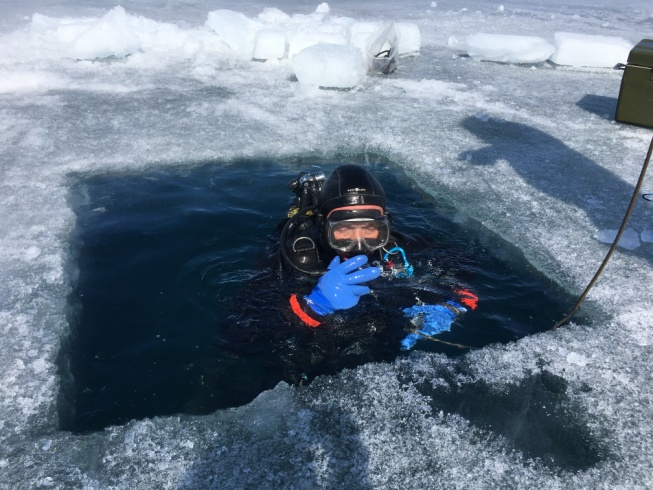
\includegraphics[height=2.23in]{media/image1.jpeg}\quad
  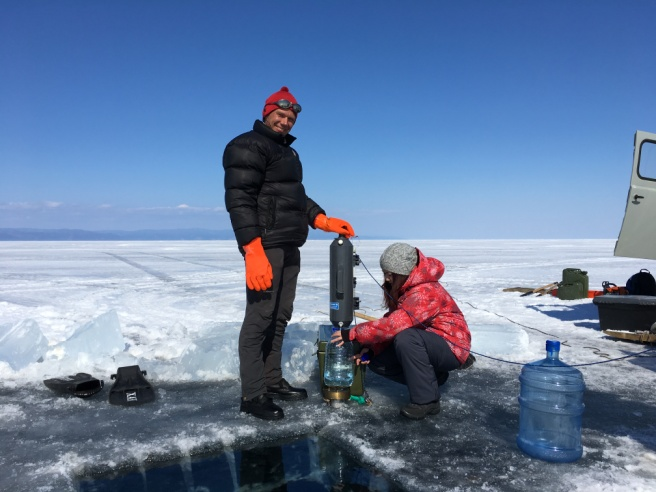
\includegraphics[height=2.23in]{media/image2.jpeg}
  \caption{ Отбор  проб  воды  в  ледовый  период }\label{fig:photo1}
\end{figure}

\begin{table}
\caption{Календарь отбора проб на различных станциях озера Байкал в
течение \theyear~г.}\label{table:1}
\begin{center}
  \newcolumntype{t}{>{\tt}c<{\relax}}
{\small%
\begin{tabular}{|l|l|l|l|l|l|l|}
  \hline
\rm Станция отбора проб & Март & Апрель & Май & Июнь & Июль &
                                                          Сентябрь\tabularnewline
                                                          \hline
Маритуй-Солзан & & & 26.05 & & 18.07 & 02.09\tabularnewline
Листвянка-Танхой &
29.03 &
12.04 &
27.05 &
06.06 &
\makecell[tl]{10.07\\
19.07}&
\makecell[tl]{03.09\\
14.09}\tabularnewline
Красный Яр-Харауз  & & & 29.05 & & 20.07 & 04.09\tabularnewline
Ухан-Тонкий        & & & 30.05 & & 26.07 & 11.09\tabularnewline
Елохин-Давша       & & & & 01.06 & 22.07 & 07.09\tabularnewline
Байкальская-Турали & & & & 02.06 & 23.07 & 07.09\tabularnewline
Баргузинский  залив  & & & 31.05 & & 25.07 & 08.09\tabularnewline
Чивыркуйский залив & & & & 04.06 & 25.07 & 08.09\tabularnewline
Пролив Малое Море  & & & & 05.06 & 21.07 & 05.09\tabularnewline
\hline
\end{tabular}%
}
\end{center}
\end{table}

Пробы отобраны для химического анализа, для подсчета численности и биомассы фитопланктона, общей численности бактерий, численности культивируемых гетеротрофов на среде РПА:10. Для определения таксономического состава про- и эукариот методом высокопроизводительного секвенирования биомассу из проб осаждали на поликарбонатные (Whatman, США) и/или ацетатцелюллозные фильтры (Владипор, Россия) 47 мм с диаметром пор 0,2~мкм с помощью прибора для вакуумной фильтрации ПВФ~47 (Россия) и вакуумного насоса НВМ-0.33II (Россия), затем смывали в ТЕ-буфер и замораживали –70~ºС до выделения ДНК.

\section{Микроскопический и микробиологический анализ проб}

Для определения общей численности и биомассы фитопланктона отбирается 100~мл пробы, производится фиксация раствором Люголя (конечная концентрация KI~--~0.66~\%, I2~--~0.33~\%) (Садчиков, 2003). Концентрацию\MA{r}{Не понятно, что делается с концентрацией?} проб проводится методом отстаивания и последующего сифонирования до объема 30~мл. Подсчет микроводорослей проводили на световом микроскопе Axiostar Plus (Zeiss, Германия) при увеличении в ×200 и ×400 раз в трех повторностях. Численность рассчитывается по методике Кузьмина (Кузьмин, 1975). Биомасса рассчитывается по методу «истинного объема» клеток (Макарова, Пичкилы, 1970; Белых и др., 2011), объем клетки каждого вида водорослей устанавливается по средним размерам, измеренным по микрофотографиям (программа Axiovision, Carl Zeiss, Germany). Определение видового состава микроводорослей и динофлагеллят проводится по атласам"=определителям (Белых и др., 2011; Поповская и др., 2011).

Для определения видового состава диатомовых водорослей пробы обрабатываются 30~\% раствором перекиси водорода при 80~°С в термостате в течение 2~ч, после чего оставляются на ночь в выключенном термостате, осадок пятикратно промывается дистиллированной водой с последующим центрифугированием при 13200~об./мин (Mini Spin, Eppendorf, Germany). Материал наносится на столик для СЭМ и напыляется золотом в вакуумной установке SDC~004 (Balzers, Liechtenstein). Препараты анализируются на сканирующем электронном микроскопе FEI Company Quanta 200 (FEI Company, USA).


По данным микроскопического анализа (рисунок~\ref{fig:micro}) на станции Листвянка"=Танхой в конце марта на нижней границе льда доминировали зеленые водоросли \emph{Chlorella vulgaris} Beyerinck {[}Beijerinck{]}, в состав пробы также входили \emph{Monoraphidium griffithii} (Berkeley) Komárková"=Legnerová\emph{, Chrysochromulina parva} Lackey\emph{, Dinobryon cylindricum} O.E.Imhof\emph{, Gymnodinium baicalense} N.L.Antipova\emph{, G. helveticum} Penard\emph{, Synedra acus} subsp.  \emph{radians} (Kütz.) Skabitsch\emph{, Rhodomonas pusilla} (H.Bachmann) Javornicky и мелкие центрические диатомеи. Общая численность микроводорослей составляла 1585,45×10\textsuperscript{3}~кл./л; общая биомасса -- 1,38~г/м\textsuperscript{3}. В составе интегральной подледной пробы доминировали зеленые водоросли \emph{M. griffity}. В пробе также были представлены диатомеи \emph{S. acus} subsp. \emph{radians, Nitzschia graciliformis} Lange"=Bertalot \& Simonsen\emph{, Cyclotela minuta} (Skvortzov) Antipova\emph{,} хризофитовые \emph{Ch. Parva, D.  cylindricum,} динофитовые \emph{G.~Baicalense, G.~Helveticum, Glenodinium apiculatum} Ehrenberg\emph{, Peridinium baicalense} Kiselev~\& Cvetkov и мелкие центрические диатомеи. Общая численность составляла 530,87×10\textsuperscript{3}~кл./л; общая биомасса -- 0,565~г/м\textsuperscript{3}. В начале апреля на нижней границе льда доминировали зеленые водоросли \emph{C. vulgaris}, в состав пробы также входили \emph{M. griffity, Ch. parva, D. cylindricum, G. baicalense, G.  helveticum, P. baicalense, P. euryceps, Aulacoseira islandica} (Otto Müller) Simonsen\emph{, S. acus, Synedra ulna} subsp\emph{. danica} (Kütz.) Skabitsch\emph{, N. graciliformis, C. minuta, R. pusilla, Сryptomonas ovata} Ehrenberg и мелкие центрические диатомеи.


Общая численность микроводорослей составляла 1647,34×10\textsuperscript{3}~кл./л; общая биомасса -- 2,388~г/м\textsuperscript{3}. В интегральной пробе подледой воды доминировали зеленые водоросли \emph{M. griffity} и диатомея \emph{S.  acus}. В состав пробы также входили \emph{S. ulna, N. graciliformis, C.  minuta, G. baicalense, G. helveticum, Gl. apiculatum, P. baicalense, M.  arcuatum, Ch. parva, D. cylindricum, R. pusilla, Сr.ovata} и мелкие центрические диатомеи. Общая численность составляла 442,85×10\textsuperscript{3}~кл./л; общая биомасса -- 0,471~г/м\textsuperscript{3}.

\begin{figure}\centering
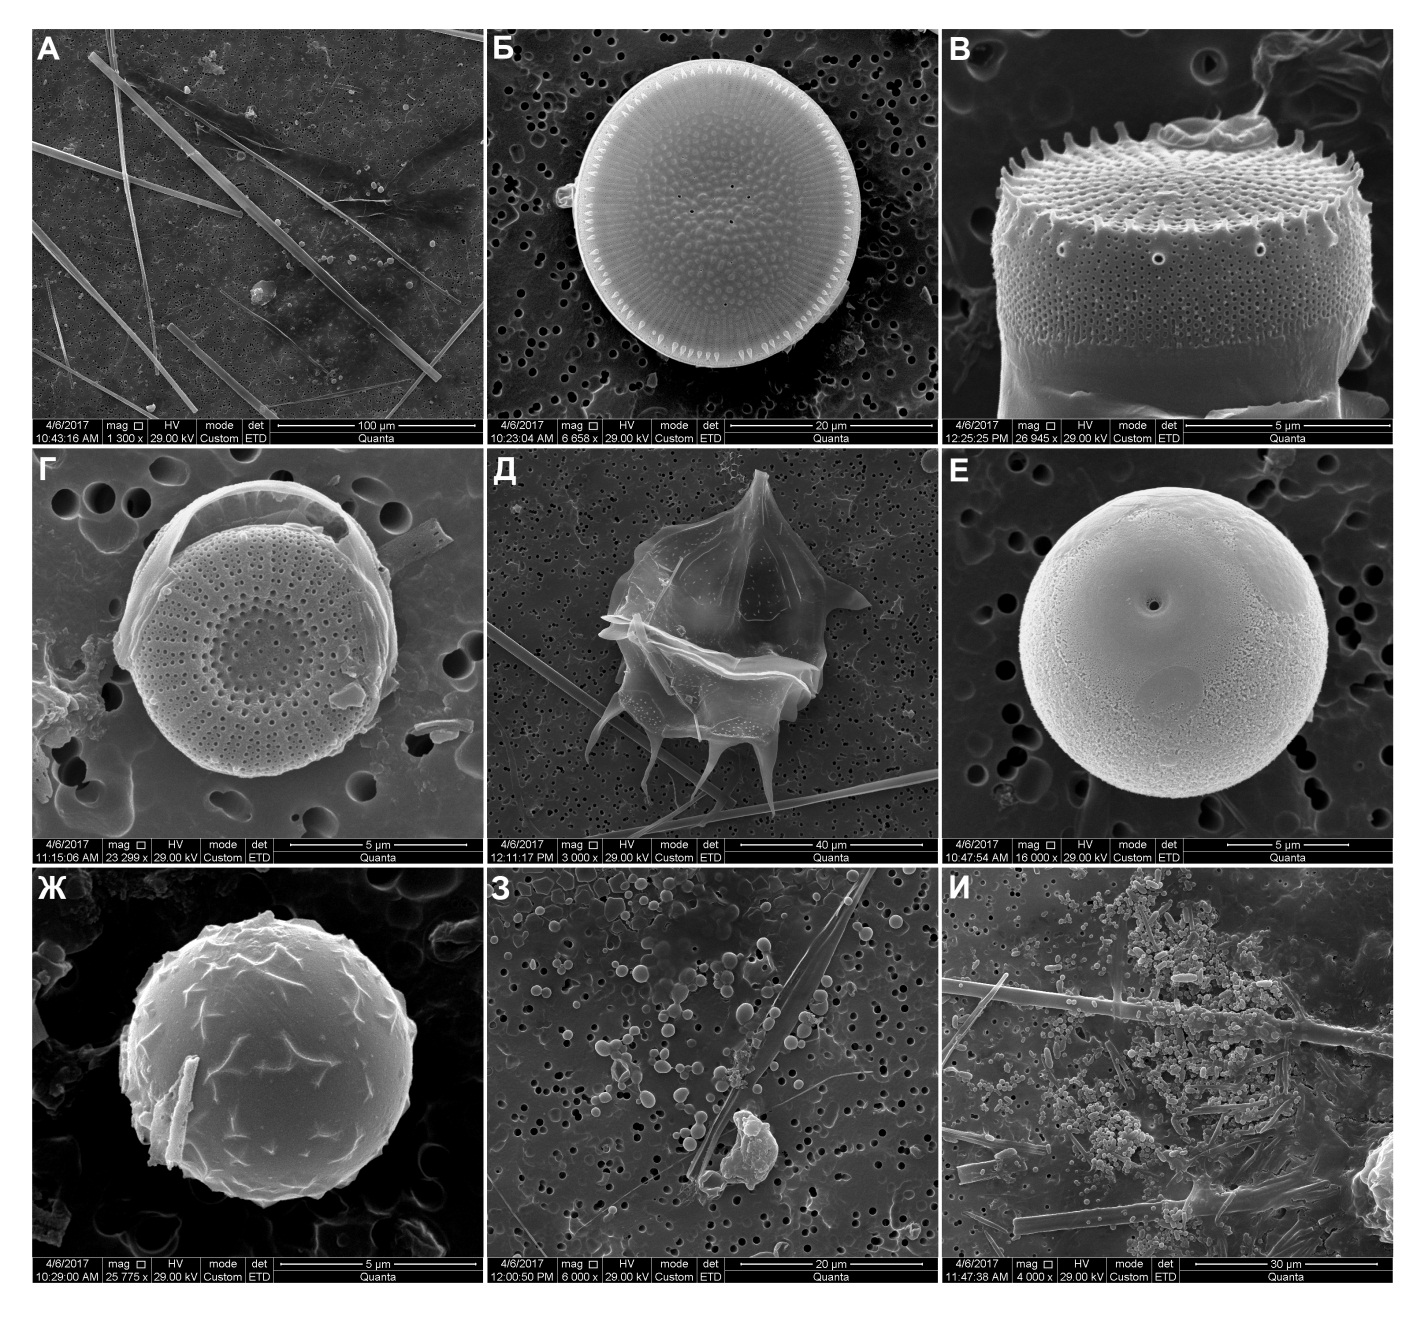
\includegraphics[width=\linewidth]{media/image3.jpeg}

\caption{Сканирующая электронная микроскопии, Листвянка"=Танхой (интегральная проба 0~--~25~м): а~--~\textit{Synedra ulna}; б~--~\textit{Cyclotella minuta}; в~--~\textit{Stephanodiscus meyeri}; г~--~мелкая центрическая диатомовая водоросль; д~--~\textit{Peridinium baicalense}; е,~ж~--~цисты хризофитовых водорослей; з,~и~--~бактерии, колонизирующие клетки микроводорослей.}\label{fig:micro}
\end{figure}

Количество гетеротрофных бактерий (КОЕ/мл) определено высевом проб на агаризованную среду РПА/10 (Горбенко и др., 1992). В верхнем слое 0--25~м воды на станции Листвянка"=Танхой эти значения варьировали (таблица~\ref{table:2}).

\begin{table}
  \caption{Количество гетеротрофных бактерий (КОЕ/мл), культивируемых на среде РПА/10, на станции Листвянка"=Танхой в мае"=июле и сентябре 2017~г.}\label{table:2}

{\tt\small%
  \setlength{\extrarowheight}{-0.2em}
  \begin{tabular*}{\textwidth}{|c|r|@{\extracolsep{\fill}}r|}
\hline
\rm Дата отбора проб & \BC{4cm}{\centering\rm Глубины, м} & \BC{0.45\textwidth}{\rm\centering Количество КОЕ/мл, среднее\\[-0.2em] для двух
повторов}\\
\hline
\multirow{7}{*}{29.03.2017} & \rm нижняя граница льда & 21,00\tabularnewline
& 0 & 19,70\tabularnewline
& 5 & 7,00\tabularnewline
& 10 & 9,50\tabularnewline
& 15 & 7,70\tabularnewline
& 20 & 5,70\tabularnewline
  & 25 & 8,00\tabularnewline
         \hline
\multirow{7}{*}{12.04.2017} & \rm нижняя граница льда & 267,30\tabularnewline
& 0 & 1,30\tabularnewline
& 5 & 1,70\tabularnewline
& 10 & 5,30\tabularnewline
& 15 & 5,00\tabularnewline
& 20 & 2,70\tabularnewline
  & 25 & 7,30\tabularnewline
         \hline
\multirow{6}{*}{27.05.2017} & 0 & 60,00\tabularnewline
& 5 & 146,50\tabularnewline
& 10 & 650,00\tabularnewline
& 15 & 205,00\tabularnewline
& 20 & 139,00\tabularnewline
& 25 & 10,50\tabularnewline
         \hline
\multirow{6}{*}{06.06.2017} & 0 & 324,50\tabularnewline
& 5 & 706,00\tabularnewline
& 10 & 1030,50\tabularnewline
& 15 & 901,50\tabularnewline
& 20 & 1930,00\tabularnewline
& 25 & 845,50\tabularnewline
         \hline
\multirow{6}{*}{10.07.2017} & 0 & 2,00\tabularnewline
& 5 & 90,50\tabularnewline
& 10 & 115,00\tabularnewline
& 15 & 82,50\tabularnewline
& 25 & 59,50\tabularnewline
         \hline
\multirow{6}{*}{03.09.2017} & 0 & 67,00\tabularnewline
& 5 & 17,00\tabularnewline
& 10 & 29,50\tabularnewline
& 15 & 293,55\tabularnewline
& 20 & 411,50\tabularnewline
& 25 & 158,50\tabularnewline
         \hline
\multirow{6}{*}{14.09.2017} & 0 & 11,00\tabularnewline
& 5 & 24,00\tabularnewline
& 10 & 175,50\tabularnewline
& 15 & 161,00\tabularnewline
& 20 & 162,00\tabularnewline
& 25 & 303,50\tabularnewline
\hline
\end{tabular*}}
\end{table}

В интегральных пробах воды, отобранных из разных районов в период с 27 мая по 5~июня также была определена общая численность бактерий.  Максимальное значение получено для пробы, отобранной на станции Маритуй"=Солзан, минимальное -- на станции Листвянка"=Танхой (рисунок~\ref{fig:chart}).

\begin{figure}
  \centering
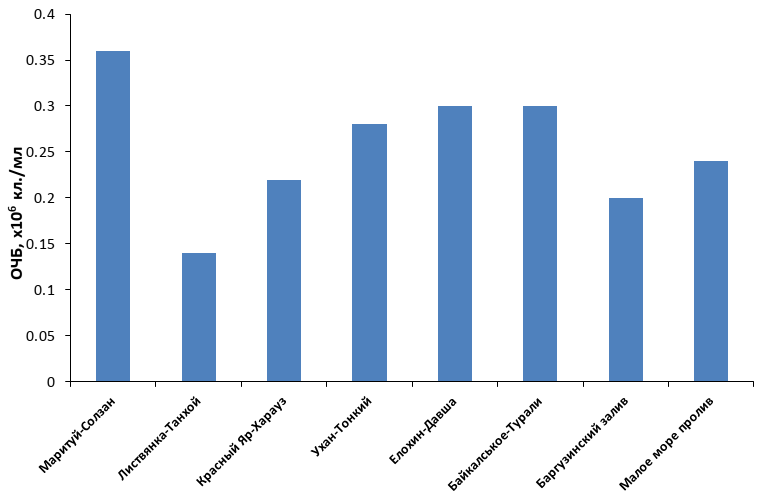
\includegraphics[width=0.8\linewidth]{media/chart.png}
\caption{ОЧБ в интегральных пробах воды (0--25~м) на станциях Байкала в мае"=июне 2017~г}\label{fig:chart}
\end{figure}


Помимо указанных выше образцов, для секвенирования на платформе Illumina MiSeq подготовлено 29 образцов ДНК из водной толщи и донных отложений Северного Байкала. Предварительно подобраны ПЦР условия и получены ПЦР продукты с бактериальными (500L, 1350R) и архейными (Arch--20F, Arch--915R) праймерами. Температурно"=временной профиль ПЦР \emph{для бактериальных праймеров} был следующим: первый цикл 94°С~--~4~мин, последующие 35~циклов 94°С~--~1~мин, 55°С~--~1~мин~10~сек, 72°С~--~1~мин~10~сек, завершающий цикл~--~72°С~--~10~мин. Для \emph{архейных праймеров} первый цикл 96°С~--~3~мин, последующие 40 циклов 96°С~--~30~сек, 50°С~--~45~сек, 72°С~--~2~мин, завершающий цикл~--~72°С~--~10~мин.  Однако не для всех образцов удалось получить библиотеки ампликонов. Наиболее вероятно, это связано с тем, что препараты суммарной ДНК из донных осадков содержали примеси, которые не позволяли успешно провести ПЦР. При выделении ДНК из осадков в будущем необходимо использовать методики и наборы, позволяющие получить препарат ДНК, свободный от ингибиторных примесей, мешающих проведению ПЦР. Также при планировании экспериментов нужно учитывать, что получение библиотек ампликонов из образцов ДНК донных осадков имеет меньшую отказоустойчивость по сравнению с образцами ДНК из проб воды.

\section{Секвенирование библиотек ампликонов 16S и 18S рРНК}

Из различных образцов воды и донных осадков подготовлено 139~библиотек ампликонов фрагментов 16S и 18S~рРНК и проведено их секвенирование с использованием высокопроизводительной платформы Illumina MiSeq в рамках выполнения работ по договору № 0334100021717000046--0009343 от 22.09.2017 по оказанию услуг с ООО~«Евраген~Лаб» (Москва). В результате суммарно получено \(\approx{}\!\!16\) миллионов парных прочтений. Медианная глубина секвенирования составила 58~тыс. прочтений на образец.

\subsection{Оценка вариабельности результатов в зависимости от использованных фильтров}

Проведена оценка уровня вариабельности результатов высокопроизводительного секвенирования и при использовании различных фильтров при отборе проб. Для этого проведен анализ слепых парных технических реплик трех библиотек. В качестве библиотек для создания реплик использованы образцы ДНК, выделенные из донных осадков и проб воды. При получении ДНК из водных образцов фильтрование бактерий осуществляли с помощью поликарбонатного и нитроцеллюлозного фильтров с диаметром пор 0,22~мкм\MA{l}{указать каких именно проб}.

Вариабельность структуры бактериальных сообществ, полученных при анализе технических реплик с помощью технологии Illumina MiSeq, находится в пределах 24-49\% (таблица~\ref{table:1-1}, рисунок~\ref{fig:1-1})\MA{r}{Это много -- или допустимо ?}.

\begin{table}
\caption{Результаты фильтрации ошибочных OTU на основании
статистического анализа равномерности встречаемости OTU в технических
репликах секвенирования бактериальных сообществ\protect\MA{r}{По-русски, и указать, какие именно это пробы}.
}\label{table:1-1}
\vspace{1em}
\centering
%\includegraphics[width=\linewidth]{media/image4.pdf}

{\small%
  \begin{tabular}[]{|c|l|c|c|c|}
\hline
\makecell{\T №\\п.п.} &\makecell[cc]{Образец, способ\\ фильтрации}&\makecell[cc]{Исходное число\\ прочтений}&\makecell[cc]{Число OTU после\\ сравнения реплик}& \makecell[cc]{Доля дискор-\\дантных OTU}\\\hline
1 &\T Water, Polycarbonare filter & 166 819 & 230 & 14\% \\
2 & Water, Celllose filter & 146 644 & 153 & 18\%\\
3 & Lake sediments, No Filter & \ \ 78 286 & 404 & 41\%\\\hline
  \end{tabular}}
\end{table}

\begin{figure}[bhtp]\centering
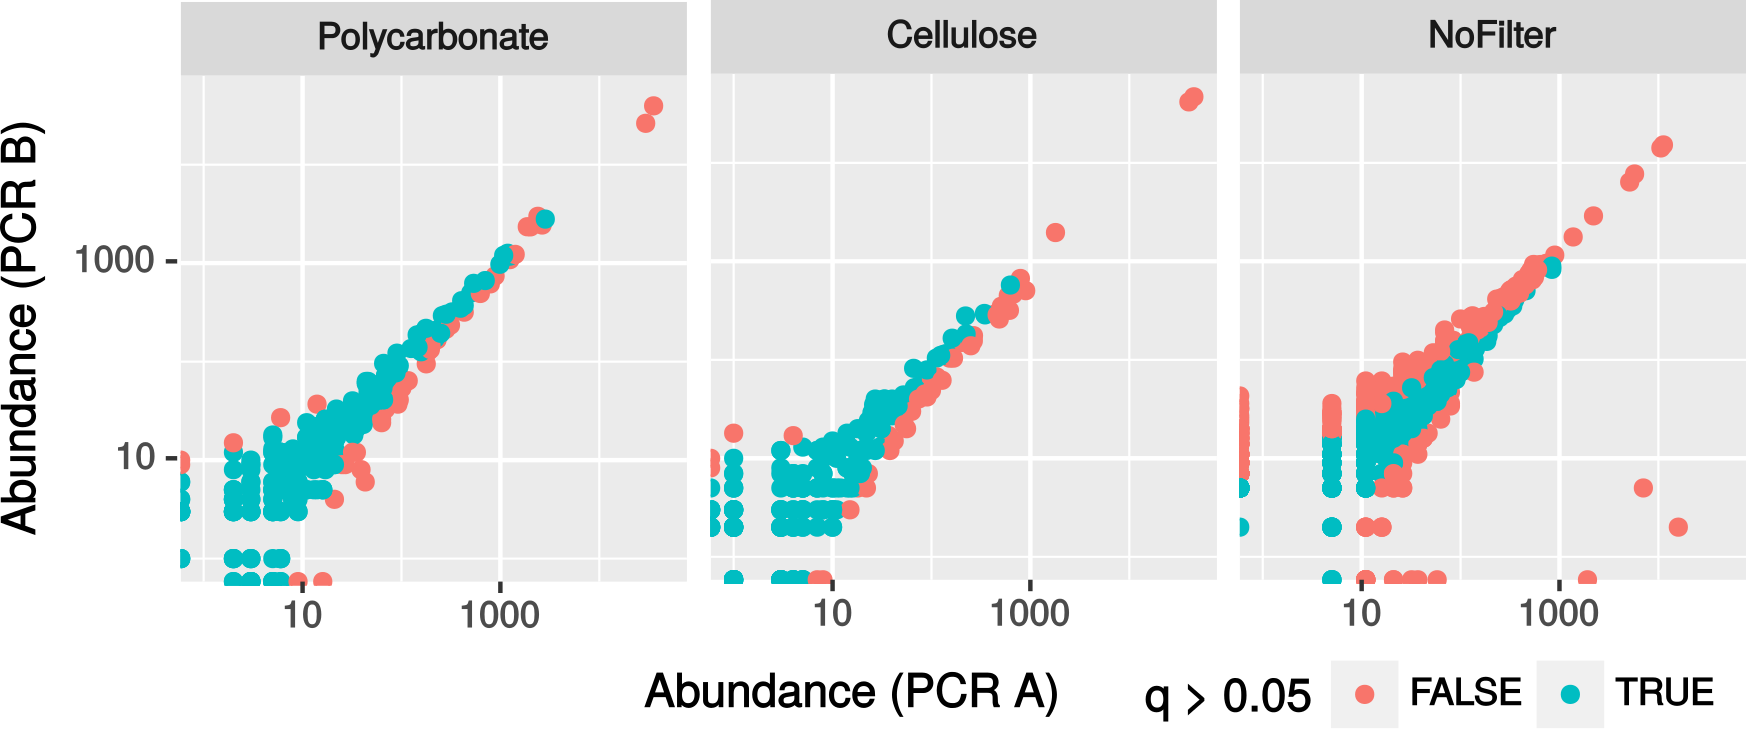
\includegraphics[width=0.9\linewidth]{media/image5.png}

\caption{FF-график, показывающий соответствие численности OTU в технических
репликах секвенирования. Красными точками отмечены OTU, встречаемость
которых различается между первой и второй репликами (Fisher's exact
test, FDR, \emph{p \textless{}} 0.05).}\label{fig:1-1}
\end{figure}

Статистический анализ показывает, что сходимость между результатами секвенирования технических реплик находится в области верхней границы допустимых значений для технологии Illumina. В частности, об этом свидетельствует высокая доля OTU, представленность которых различается между техническими репликами секвенирования при выбранном уровне значимости. Это свидетельствует о необходимости принятия дополнительных мер с целью выявления ошибочных OTU перед сравнительным анализом структуры сообществ. Одним из таких методов может быть выполнение технических реплик для каждого анализируемого ампликона и статистическая оценка равномерности представленности OTU.

Образцы №1 и 2 представляют собой суммарную ДНК бактерий, выделенных из одного образца байкальской воды с применением разных фильтров. При сравнении технических реплик выявлено, что доля дискордантных OTU при использовании целлюлозных фильтров выше, чем при использовании поликарбонатных фильтров (таблица~\ref{table:1-1}).

\begin{figure}\centering
  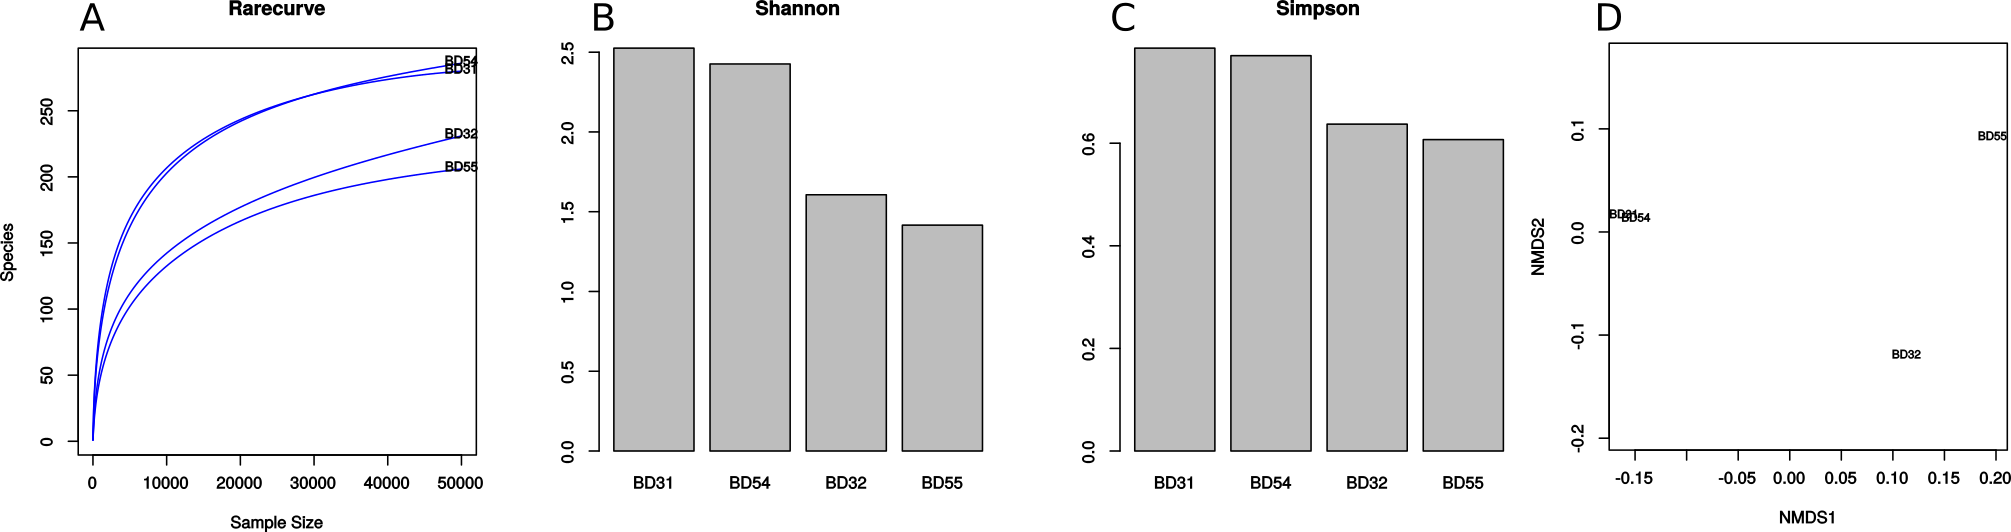
\includegraphics[width=0.9\linewidth]{media/image6.png}
  \caption{Анализ \(\alpha\)- и \(\beta\)-разнообразия сообществ, полученных при секвенировании
технических реплик №1 (BD31, BD54) и 2~(BD32 и BD55). A~--~кривые
разрежения; B~--~индексы Шеннона; C~--~индексы Симпсона, D~--~ординация
сообществ (NMDS, дистанция Bray-Curtis).}\label{fig:2}
\end{figure}


Кривые разрежения, построенные для этих сообществ, имеют разные ассимптоты (рисунок~\ref{fig:2}a), а индексы \(\alpha\)-разнообразия достоверно различаются для сообществ, №1 и №2 (Student's t-test, \emph{p} \textless{} 0.05).  Ординация сообществ показывает, что вариабельность технических реплик №2 значительна, тогда как технические реплики №1 формируют компактный кластер.

Эти \hl{результаты} свидетельствуют о том, что при использовании поликарбонатных фильтров для фильтрации бактерий из водных природных проб \hl{результаты} имеют более высокую воспроизводимость.

\chapter{Процедура тримминга метагеномных данных, полученных путем высокопроизводительного секвенирования ампликонов}\label{chap:2}

Метагеномный анализ, проводимый на основе расшифрованных последовательностей ампликонов, широко применяется для исследования таксономичнского разнообразия в сообществах микроорганизмов (Petrosino J.F., \textit{et al}, 2009; Kim M., \textit{et al}, 2013). При этом анализируют последовательности, полученные при секвенировании ампликонных библиотек 16S рРНК. При проведении подобных исследований для получения статистически достоверного результата необходимо увеличение, как длины читаемых фрагментов, так и количества последовательностей. Для оптимизации исходных данных в двух указанных направлениях часто используется технология <<Illumina>> с парными концевыми прочтениями фрагментов исходной библиотеки (Quail M.A. \textit{et al}. 2012). Критически важным фактором при выделении OTU для определения таксономического разнообразия является точность, с которой определены генетические дистанции. Искажение при расчете генетических дистанций может возникнуть при наличии ошибок -- не точно определенных в процессе секвенирования нуклеотидах. Недостатком технологии <<Illumina>>, возникающим при проведении метагеномного анализа, основанного на секвенировании ампликонных библиотек являться низкое качество прочтения. Это может привести к тому, что при выделении OTU будут возникать погрешности, искажающие результаты сравнительного анализа состава сообществ. Тримминг (фильтрация по качеству прочтения) с использованием стандартного алгоритма скользящей рамки может привести к резкому сокращению числа последовательностей, пригодных для анализа. В процессе выполнения проекта разработан алгоритм фильтрации -- триминга метагеномных данных полученных при парно''=концевом секвенировании ампликонов.  Предлагаемый алгоритм триминга способствует достижению компромисса между количеством последовательностей и длиной сравниваемых фрагментов, позволяя избежать больших потерь длинны и удаления значительного количества последовательностей повышая точность сравнительного таксономического анализа.

\section{Процедура тримминга}
Основная стратегия тримминга метагеномных прочтений ампликонной библиотеки, реализованная в предлагаемой процедуре, заключается в том, чтобы не производить удаление самой последовательности с плохим качеством прочтения из исходного набора, а удалять только некоторые позиции (столбцы) в наборе выровненных последовательностей, качество прочтения букв в которых не является удовлетворительным. При таком тримировании происходит некоторое уменьшение длины сопоставляемых фрагментов, но не происходит потеря последовательностей из анализа. При исключении в выравнивании столбцов, содержавших недостоверные буквы, уменьшается ошибка, с которой определяется генетическая дистанция.  Предлагаемая процедура тримига состоит из следующих этапов:

\begin{enumerate}
\item Сшивка парных прочтений в контиги из сырых данных. Можно провести предварительную фильтрацию исходных парных прочтений на предмет удаления слишком коротких или слишком длинных фрагментов, которые явно представляют собой ошибки секвенирования. Сшивку можно провести с помощью программы FLASH (Magoč T., Salzberg S.L., 2011), которая рекомендуется в некоторых работах для объединения парных концевых прочтений ампликонов (Fosso B., \textit{et al}, 2015; Tennant R.K., \textit{et al}, 2017).

\item Конвертирование сшитых прочтений из формата fastq в формат fasta и выравнивание последовательностей. Для выравнивание можно рекомендовать один из распространенных алгоритмов, например MAFT (Katoh K., Toh H., 2010). При выравнивании последовательностей маркеров 18S и 16S~рРНК рекомендуется использовать программу MOTHUR (Schloss P.D., \textit{et al}, 2009) и референсную базу данных SILVA (Quast C., \textit{et al}, 2013).

\item Сопоставление информации о качестве прочтения букв из файла формата fastq, соответствующим буквам в выровненном наборе последовательностей.  Буквам сопоставляться информация о качестве прочтения, пробелам никакой информации не сопоставляется.

\item Задание критического порога по качеству для удаления позиции из выравнивания.

\item Задание критического порога по доли позиций с качеством ниже критического для удаления позиций из элаймента.

\item Определение номеров позиций в элайменте отвечающих условию удаления.

\item Удаление позиций, соответствующих выбранным номерам из элаймента.
\end{enumerate}

Пункты с 3 по 7 реализованы в виде программы на языке программирования R с применением пакета ShortRead (Morgan, M., \textit{et al} 2009). Программа включает в себя три функции: 1) функция для визуализации доли букв в позиции выравнивания с качеством ниже критического; 2) Функция для тримига -- удаление позиций с заданной долей позиций с качеством ниже критического; 3) функция для дополнительно триминга -- удаление последовательностей содержавших некачественные позиции в начале и в конце прочтения, аналогично процедуре стандартного тримминга.

При проведении тримминга стандартный порог для качества прочтения позиции равный 20 единиц соответствует вероятности ошибочного определения нуклеотида в 0.1 и порогу удаления позиции из выравнивания равному 0.1, что соответствует наличию в позиции выравнивания 10\% букв с качеством меньшим, чем 20 единиц.

\section{Тестирование процедуры тримминга}

Для тестирования предлагаемой процедуры тримминга ампликонных данных использован набор последовательности участка гена 16S~рРНК сообщества бактерий выделенных из водного образца. Амплификация проводилась, используя эубактериальные праймеры 9F и 541R, фланкирующие участок V1--V3 гена 16S~рРНК (Chun, J., \textit{et al}, 2010).

Сборка парно концевых прочтений в контиги проводилась с помощью программы FLASH (Magoč T., Salzberg S.L., 2011). Стандартный тримминг контигов по качеству прочтения проводился с помощью Trimmomatic (Bolger A.M., \textit{et al}. 2014). Триммированный и не треммированый наборы последовательностей выравнивались с помощью программы MOTHUR и базы данных SILVA. С помощью MOTHUR и SILVA из выровненных наборов данных удалены химерные последовательности, последовательности, не идентифицированные как бактериальные и последовательности, не выравнивающиеся на участок V1--V3 гена 16S рРНК. Набор выровненных нетреммерованных последовательностей отфильтрован по предложенной методике тримминга.

Для двух наборов выровненных последовательностей, триммированных по стандартной и прилагаемой в работе методике, проведен анализ с выделением OTU уровне кластерного расстояния 0.03 -- уровень вида при сравнении 16S~рРНК. Выделанные OTU отсортированы по убыванию представленности в бактериальном сообществе. Отдельно рассматривались наборы OTU доминирующих в исследуемом сообществе таксонов бактерий, составляющих 95\% пула расшифрованных последовательностей. Для каждого из OTU определены репрезентативные последовательности -- последовательности с наименьшим средним генетическим расстоянием до других последовательностей в OTU. Сопоставление репрезентативных последовательностей позволило идентифицировать одинаковые OTU в двух видах анализа. Расчет \hl{дистанций кластеризации} и выделений OTU проводился с помощью программы MOTHUR (Schloss P.D., \textit{et al}, 2009). Идентификация бактериальных OTU до уровня рода проводилась путем сопоставления последовательностей с референсной базой данных SILVA (Quast C., \textit{et al}, 2013).

Статистическая сходимость результатов метагономномного анализа на основе выделенных OTU оценивалась с помощью кривых насыщения и бутстреп"=индекса (Smith E.P., van Belle G, 1984), оценивающего количество недооцененных таксонов в исследуемом наборе данных. Расчеты проводились с помощью пакета vegan (Dixon P., 2003) для языка программирования R.

\section{Анализ и интерпретация результатов применения тримминга}

Первичный набор данных расшифрованных последовательностей ДНК содержал 26987 парных прочтений.  Доля букв в некоторых позициях прочтений с качеством прочтения ниже 20 единиц возрастает к концу каждого прочтения из пары и достигает 25\%.  После сшивки получено 18870 контигов. При стандартном тримминге в программе Trimmomatic количество контигов сократилось до 4435. После триминга в наборе данных уменьшилась доля более длинных последовательностей и увеличилась доля более коротких фрагментов. Более длинные контиги имели в среднем больший провал по качеству определения нуклеотидов в области сшивки (средняя часть контигов), благодаря чему при стандартном тримминге длинные контиги в большей степени элиминировались из набора данных.

Результаты кластеризации и выделения OTU, проведенные на основе наборов последовательности, триммированных двумя способами представлены в таблице~\ref{table:3-1}. При стандартном тримминге количество доминирующих OTU равнялось 184, а при тримминге с помощью предлагаемого алгоритма 319. При стандартном тримминге ожидаемое количество OTU с учетом недооцененных OTU равнялось 291, а при предлагаемом способе тримминга 499. В силу того, что два исследуемых набора последовательностей характеризуют одно и то же сообщество бактерий (одну и ту же генеральную совокупность), оценочные характеристики ожидаемого количества доминирующих OTU должны быть близкими по значению. Так как при стандартном тримминге в наборе присутствовало 3840 последовательности, а при предлагаемой схеме тримминга 17160 последовательной, ожидаемая доля недооцененных доминирующих OTU в первом случае должна быть больше чем во втором. В рамках проводимого анализа доли недооцененных OTU оказалась одинаковой и равнялась 63\%. Определенные таким образом показатели разнообразия говорят о том, что в случае стандартного тримминга произошло обеднение таксономического состава сообщества. При стандартном тримминге не происходит селективно нейтральной элиминации последовательностей из набора данных.

\begin{table}
  \centering
  \caption{Показатели разнообразия таксономического состава сообществ при метогеномном анализе, основанном на выделении OTU}\label{table:3"=1}

{\tt\small
\begin{tabular}[]{|>{\rm\raggedright}p{0.4\textwidth}|c|c|}
  \hline
\makecell[cc]{\rm\bfseries\\[-0.3em]\bf{}Наименование показателя} & \multicolumn{1}{p{3cm}|}{\rm\centering\bfseries Стандартный триминг} &
\multicolumn{1}{p{3cm}|}{\rmfamily\centering\bfseries{}Специальный триминг}\tabularnewline\hline
\T Наблюдаемое количество OTU & 405 & 1199\tabularnewline\hline
Количество не синглетных OTU & 268 & 567\tabularnewline\hline
Количество синглетных OTU & 137 & 632\tabularnewline\hline
\makecell[cl]{Доля последовательностей в\\ синглетных OTU} &\multirow{1}{*}{0.036} &\multirow{1}{*}{0.037}\tabularnewline\hline
\makecell[cl]{Количество доминирующих OTU\\
(95\% sample size)} &\multirow{1}{*}{184}&\multirow{1}{*}{319}
\tabularnewline\hline
\makecell[cl]{Ожидаемое количество доминирующих\\ OTU (95\% sample size)\\ (Bootstrap index)}&\multirow{1}{*}{291}&\multirow{1}{*}{499}\\\hline
\makecell[cl]{Отношение наблюдаемого количества\\ доминирующих OTU к ожидаемому\\
доминирующих количеству OTU} &\multirow{1}{*}{0.63} &\multirow{1}{*}{0.63}\tabularnewline\hline
\makecell[cl]{Индекс Шеннона для доминирующих\\ OTU
(95\% sample size)}&\multirow{1}{*}{4.23}&\multirow{1}{*}{4.93}\\
\hline
\end{tabular}}
\end{table}


Построенные кривые насыщения \hl{ведами} (насыщения OTU), представленные рисунке~\ref{fig:3-1}, показывают картину, аналогичной той, которая наблюдается при анализе показателей биологического разнообразия (см.~таблицу~\ref{table:3-1}). Кривые насыщения выходят на плато на разных уровнях количественной представленности OTU. Кривые насыщения, построенные по статистике представленности OTU, полученной при анализе выборки после стандартного триммера, выходят на плато на уровнях 184 (95\% доминирующий пул OTU) и 268 (полный пул последовательностей). При анализе выборки после предлагаемого в работе способа тримминга кривые насыщения выходят на плато на уровнях 319 (95\% доминирующий пул OTU) и 567 (полный пул последовательностей). Так как после стандартного тримминга набор содержал меньше последовательностей, можно было бы предположить, что кривые насыщения для анализа, проведенного на его основе, не должны выходить на плато в принципе, \hl{а} стремиться к величинам характерным для анализа, проделанного на большем количестве данных. Все это свидетельствует в пользу того, что при стандартном тримминге произошло обеднение таксономического разнообразия в спектре оставшихся после фильтрации последовательностей.

\begin{figure}\centering
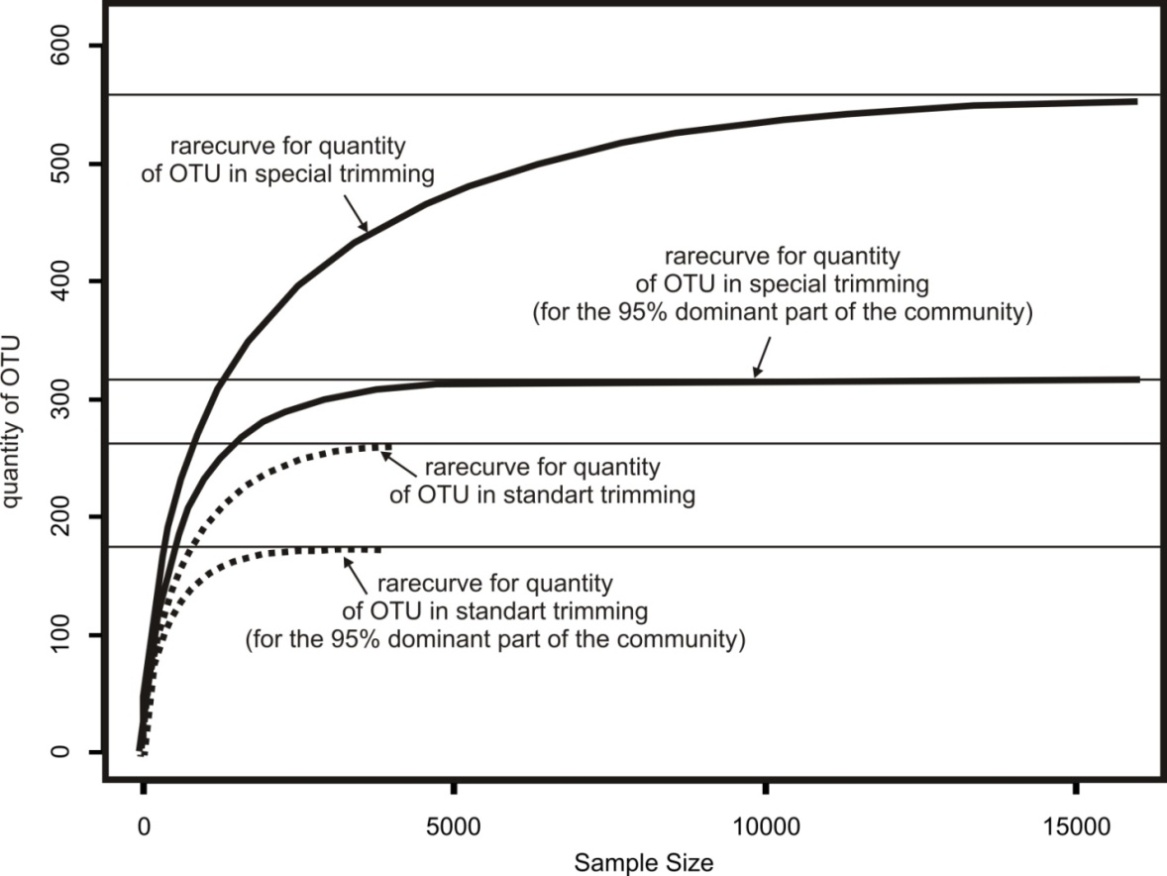
\includegraphics[width=0.6\linewidth]{media/image7.jpeg}

\caption{Кривые насыщения количества OTU}\label{fig:3-1}
\end{figure}

Таким образом, в ходе реализации данной части проекта установлено, что при обработке данных, полученных в ходе высокопроизводительного секвенирования ампликонов необходимо более аккуратно подходить к процедуре фильтрации исходного набора данных по качеству прочтения. В ходе использования стандартной процедуры тримминга происходит смешение представленности последовательностей различных таксономических групп в наборе данных. Для решения проблемы предлагается процедура триммирования последовательностей, предотвращающая таксономические искажения в наборе данных. Кроме того, предлагаемая процедура фильтрации позволяет избежать потере значительного количества последовательностей и достичь более достоверного результата статистического сопоставления таксономического разнообразия в сравниваемых пробах.

\chapter{Метагеномный анализ сообществ бактерий в подледной воде} \label{chap:3}

Совместно с Группой эволюционной геномики Университета им. Мигеля
Эрнандеса (Испания) впервые проведен метагеномный анализ геномов (MAG)
микроорганизмов в двух образцах из трофогенного слоя (5 и 20 м) Южного
Байкала в подледный период. На основании анализа структуры гена 16S рРНК
из MAG в отличие от других водных экосистем в планктоне Байкала отмечена
необычайно высокая доля бактерий филума \emph{Verrucomicrobia}, тогда
как широко распространенные представители филумов \emph{Actinobacteria}
и \emph{Proteobacteria}, имели пропорции, аналогичные для сообществ из
других озер (рисунок~\ref{fig:4-3}).

\begin{figure}\centering
  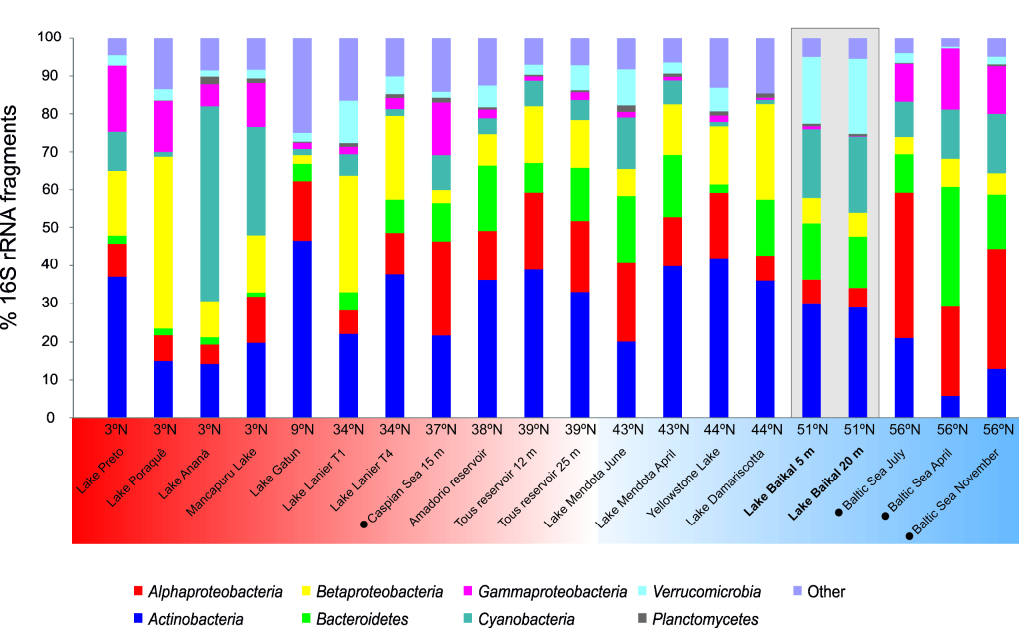
\includegraphics[width=\linewidth]{media/image8.png}
  \caption{Структура прокариотических сообществ на основе анализа
структуры гена 16S рРНК из несобранных метагеномов озера Байкал (образцы
с 5 и 20 м) и данными для пресноводных и солоноватых водоемов,
расположенных на широтах от 0 до 56º. Все данные получены
непосредственно из метагеномов (без амплификации). Представлены данные
из озер от экваториальных и умеренных до холодноводных широт. Градиент
от красного до синего показывает широты различных пресноводных и
солоноватых водоемов, используемых для сравнения. Данные из солоноватых
экосистем обозначены черной точкой, данные озера Байкал выделены жирным
шрифтом.}\label{fig:4-3}
\end{figure}

Отличительной чертой геномов байкальских бактерий (и, возможно, клеток)
являются их небольшие размеры (\textless{} 2.7 Mb для
\emph{Actinobacteria, Bacteroidetes, Thaumarchaeota, Cyanobacteria} и
некоторых \emph{Verrucomicrobia}). Метагеномный анализ полных геномов
свидетельствует о наличии новых линий, которые практически не
встречаются в других водоемах и имеют лишь отдаленное родство с геномами
MAG других пресноводных микроорганизмов.

Впервые собрано и проанализировано 11 новых геномов SAR11 одного из
наиболее часто встречающихся в мире таксонов филума
\emph{Alphaproteobacteria} (Giovannoni \textit{et al}. 1999; Morris \textit{et al}.,
2002). Анализ данных показал (рисунок~\ref{fig:4-4}), что часть геномов байкальских
микроорганизмов сходна с геномами из других пресноводных озер и
водохранилищ, в частности с геномами микроорганизмов из солоноватого и
холодноводного Балтийского моря. Среди 35 реконструированных геномов в
15 MAGs отмечены гены родопсина (рисунок~\ref{fig:4-5}), что может свидетельствовать
о фотогетеротрофии байкальских бактерий, несмотря на наличие толстого
ледяного/снежного покрова, препятствующего проникновению света. На
основе анализа геномов и кодирующих белков собран геном бактериофага
Polynucleophage Baikal-20-5m-C28, предполагаемым хозяином которого
являются бактерии рода \emph{Polynucleobacter}, хемогетеротрофы - широко
распространенные обитатели пресных водоемов. В геноме этого фага имеется
несколько вспомогательных метаболических генов. Предполагается, что он
способен изменять гетеротрофный метаболизм хозяина во время инфекции
(Daines \textit{et al}., 2015), подобно тому, как цианофаги перенаправляют
автотрофный метаболизм хозяина на путь, который благоприятствует
вирусной репликации.

\begin{figure}\centering
  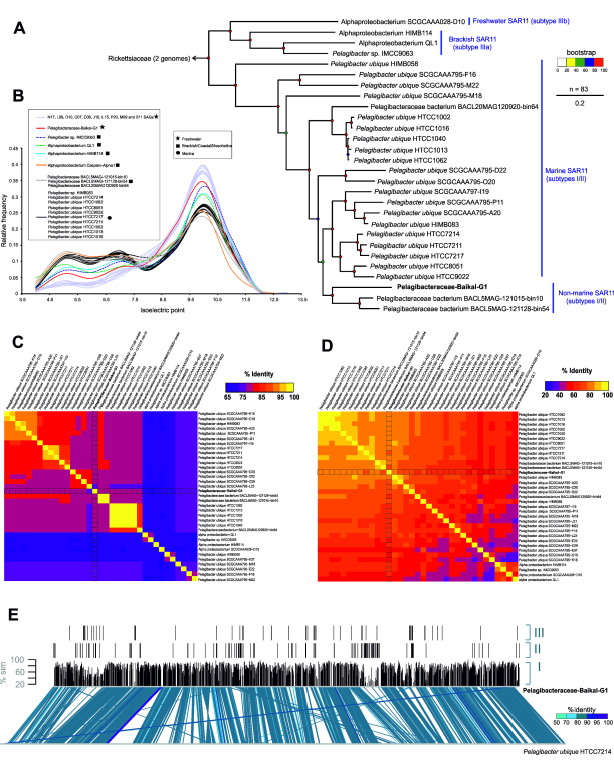
\includegraphics[width=0.8\linewidth]{media/image9.png}
  \caption{(A) Филогенетическое положение геномов SAR11 из озера Байкал
относительно представителей клад I / II, IIIa и IIIb. В качестве корня
дерева использовались два генома \emph{Ricckettsiacae}. (B). Оценка
относительных частот белка по сравнению с изоэлектрической точкой (IP)
оценивается на подмножестве представителей морских, солоноватых и
пресноводных SAR11. (C) Средняя нуклеотидная идентификация (ANI) и (D)
средняя аминокислотная идентификация (AAI) между
Pelagibacteraceae-Baikal-G1 и подмножеством репрезентативных геномов
SAR11 I / II, IIIa, IIIb. (E) Выравнивание Pelagibacteraceae-Baikal-G1 с
\emph{Pelagibacter ubique} HTCC7214 с помощью BLASTN с \textgreater{}
70\% идентичности и \textgreater{} 200 п. н. длины выравнивания. (E-I)
расположение и сходство гомологов TBLASTX, \textgreater{} 50\% и
\textgreater{} 200 п. н. длины выравнивания (E-II) локализация 120 генов
из Pelagibacteraceae-Baikal-G1, которые не соответствуют
репрезентативной \emph{Pelagibacter ubique} HTCC7214 (E- III)
расположение 51 уникального гена Pelagibacteraceae-Baikal-G1 в других
геномах I-II кластеров SAR11.}\label{fig:4-4}
\end{figure}

\begin{figure}\centering
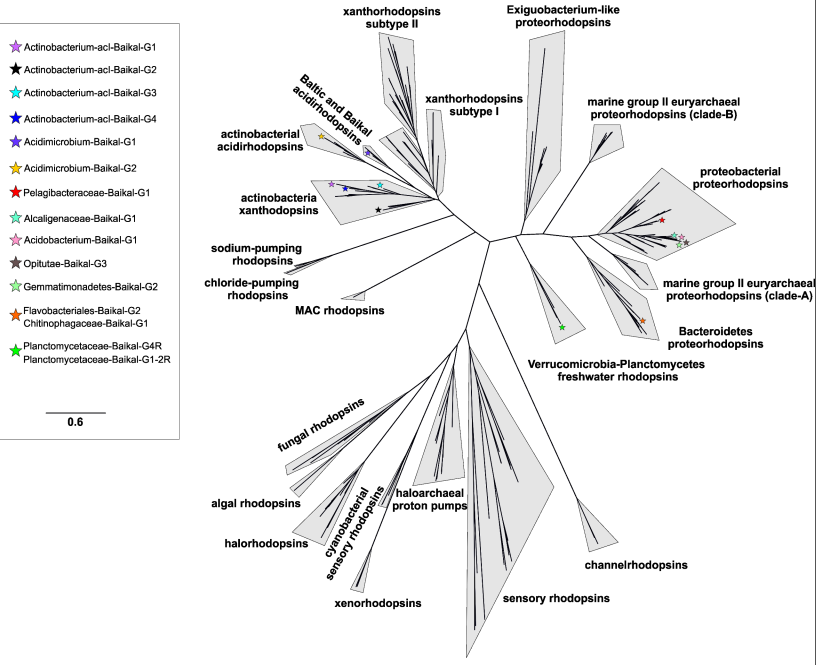
\includegraphics[width=\linewidth]{media/image10.png}

\caption{Филогенетическое дерево родопсинов, построенное с
использованием 200 репрезентативных архейных и бактериальных родопсинов.
Включены все известные типы родопсиновых клад. Принадлежность клад
разных родопсинов из MAGs озера Байкал выделена цветом и помечена
звездочкой.}\label{fig:4-5}
\end{figure}

Подобно тому, как цианофаги перенаправляют автотрофный метаболизм
хозяина на путь, который благоприятствует вирусной репликации (Daims et
al., 2015) конец предложения. Среди аннотированных белков, кодируемых в
Байкале-20-5 м-С28, были хитиназа (CDS12) и гликозидгидролаза (CDS 189).
Эти белки обладают способностью деградировать полисахариды, и, таким
образом, могут обеспечить \emph{Polynucleobacter} дополнительными
источниками энергии в ультра-олиготрофном озере Байкал (Weiss \textit{et al}.,
1991; Zeng \textit{et al}., 2014) во время фаго-литического процесса.

\begin{figure}\centering
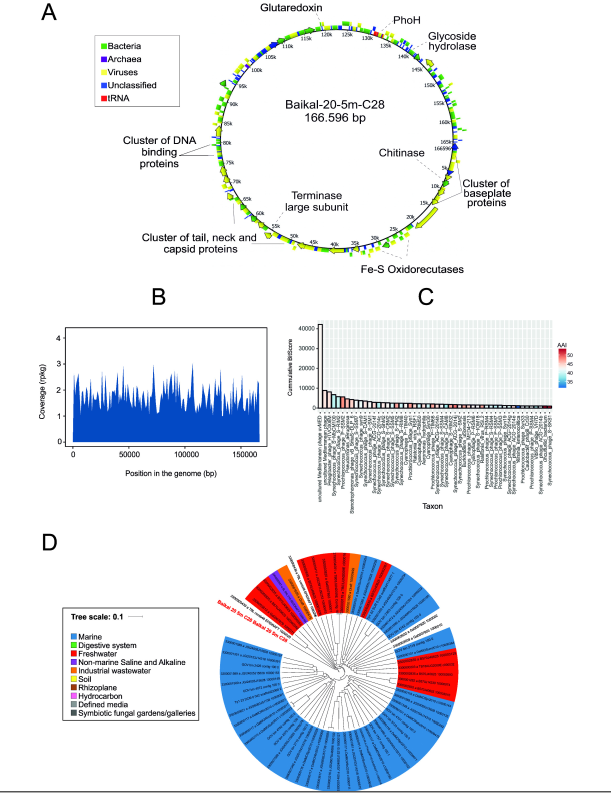
\includegraphics[width=0.8\linewidth]{media/image11.png}

\caption{Геном Polynucleophage Baikal-20-5m-C28 озера Байкал. A)
Циркулярная карта генома фага Baikal-20-5m-C28 с указанием
предполагаемых вспомогательных метаболических генов и генов, участвующих
в репликации фагов и сборке вирионов. Гены изображены стрелками и
закодированы цветом в соответствии с таксономической принадлежностью
своих ближайших гомологов в базе данных белков NCBI-NR. Модули белков,
вовлеченных в базальную пластинку, сократительный чехол, полый стержень,
связывание ДНК и капсидные белки подчёрнуты. Б) График покрытия вдоль
генома Baikal-20-5m-C28. С) Barplot, отображающий кумулятивный BitScore
и среднюю аминокислотную идентичность (AAI) между геномом
Baikal-20-5m-C28 и геномами фагов и бактерий из базы данных NCBI-NR. D)
Подмножество phylogenomic дерева Dice, отображающее размещение
Baikal-20-5m-C28 и ближайших родственников этих геномов. Ветви окрашены
в соответствии с источником экосистемы фаговых геномов.\textbf{НЕТ ССЫЛКИ ИЗ ТЕКСТА}}\label{fig:4-6}
\end{figure}

Чтобы оценить наличие собранных геномов в различных пресноводных и
солоноватых водоемах, была выполнена подборка фрагментов с
\textgreater{} 95\% значений идентичности (выше уровня видов). Для
сравнения использовалось наборы данных (\textgreater{} 150 различных),
полученные при исследовании тропических, умеренных и холодных экосистем,
а также Балтийского и Каспийского морей (Hugerth \textit{et al}., 2015; Mehrshad
\textit{et al}, 2016). Наибольшее сходство наблюдалось с данными из Балтийского
моря и из пресноводных экотопов и только по структуре генов 16S рРНК и
другим консервативным генам. С этими исключениями и выше 95\%
идентичности значительного присутствия микробов Байкала в других средах
не наблюдалось. Следовательно, большинство восстановленных геномов может
быть эндемиками Байкала, где микробы адаптированы к холодным и особым
гидрологическим и гидрохимическим условиям, существующим в этом озере.

\chapter{Регистрации выделенных в культуру бактерий}\label{chap:4}

Из донных осадков метанового сипа «Посольская Банка» изолированы два
термофильных, факультативно анаэробных штамма микроорганизмов,
отнесенных к р. \emph{Thermaerobacter} и р. \emph{Geobacillus}. Штамм
\emph{Geobacillus} sp. PB15/Grf7geo способен выдерживать широкий
диапазон температур, с оптимумом роста 55--60°С. Хемоорганогетеротроф
(рисунок~\ref{fig:5-1}).

\begin{figure}[hb]\centering
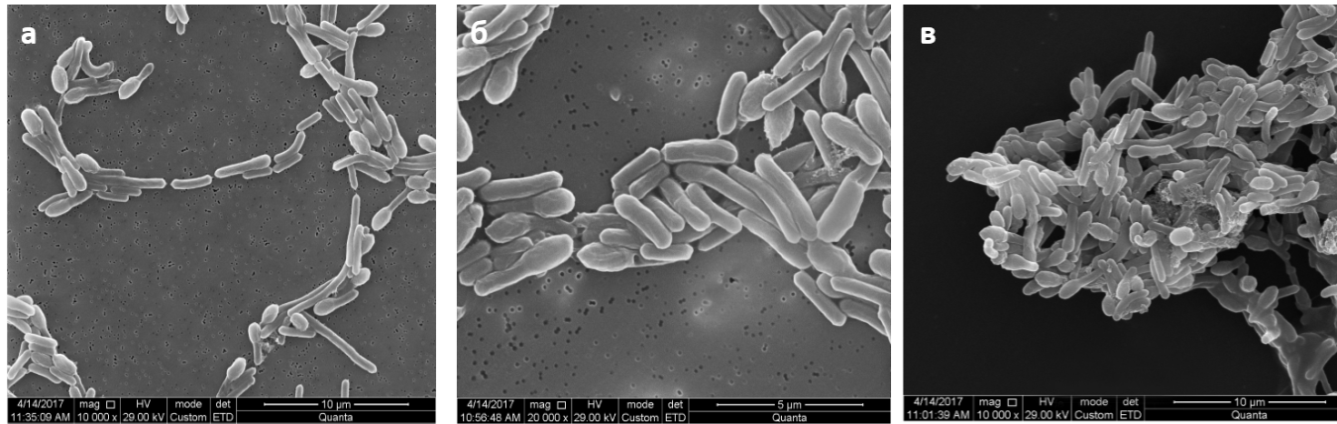
\includegraphics[width=0.9\linewidth]{media/image12.png}

\caption{Морфология клеток штамма PB15/Grf7geo на плотной
питательной среде: суточная культура (а), трехсуточная культура (б, в).
Масштаб: а, в -- 10 мкм, б -- 5 мкм}\label{fig:5-1}
\end{figure}

Несмотря на то, что термофильный, факультативно анаэробный штамм
\emph{Geobacillus} sp. PB15/Grf7geo выделен из низкотемпературного
биотопа, его физиолого-биохимические свойства не отличаются от свойств
типовых термофильных штаммов этого рода. Вместе с тем, анализ структуры
гена 16S рРНК штамма PB15/Grf7geo свидетельствует о его неполной
идентичности типовым культивируемым штаммам (97 \%) и обособленном
филогенетическом положении внутри кластера последовательностей типовых
видов (рисунок~\ref{fig:5-2}). Последние результаты являются основанием для отнесения
полученного штамма к новому виду.

\begin{figure}\centering
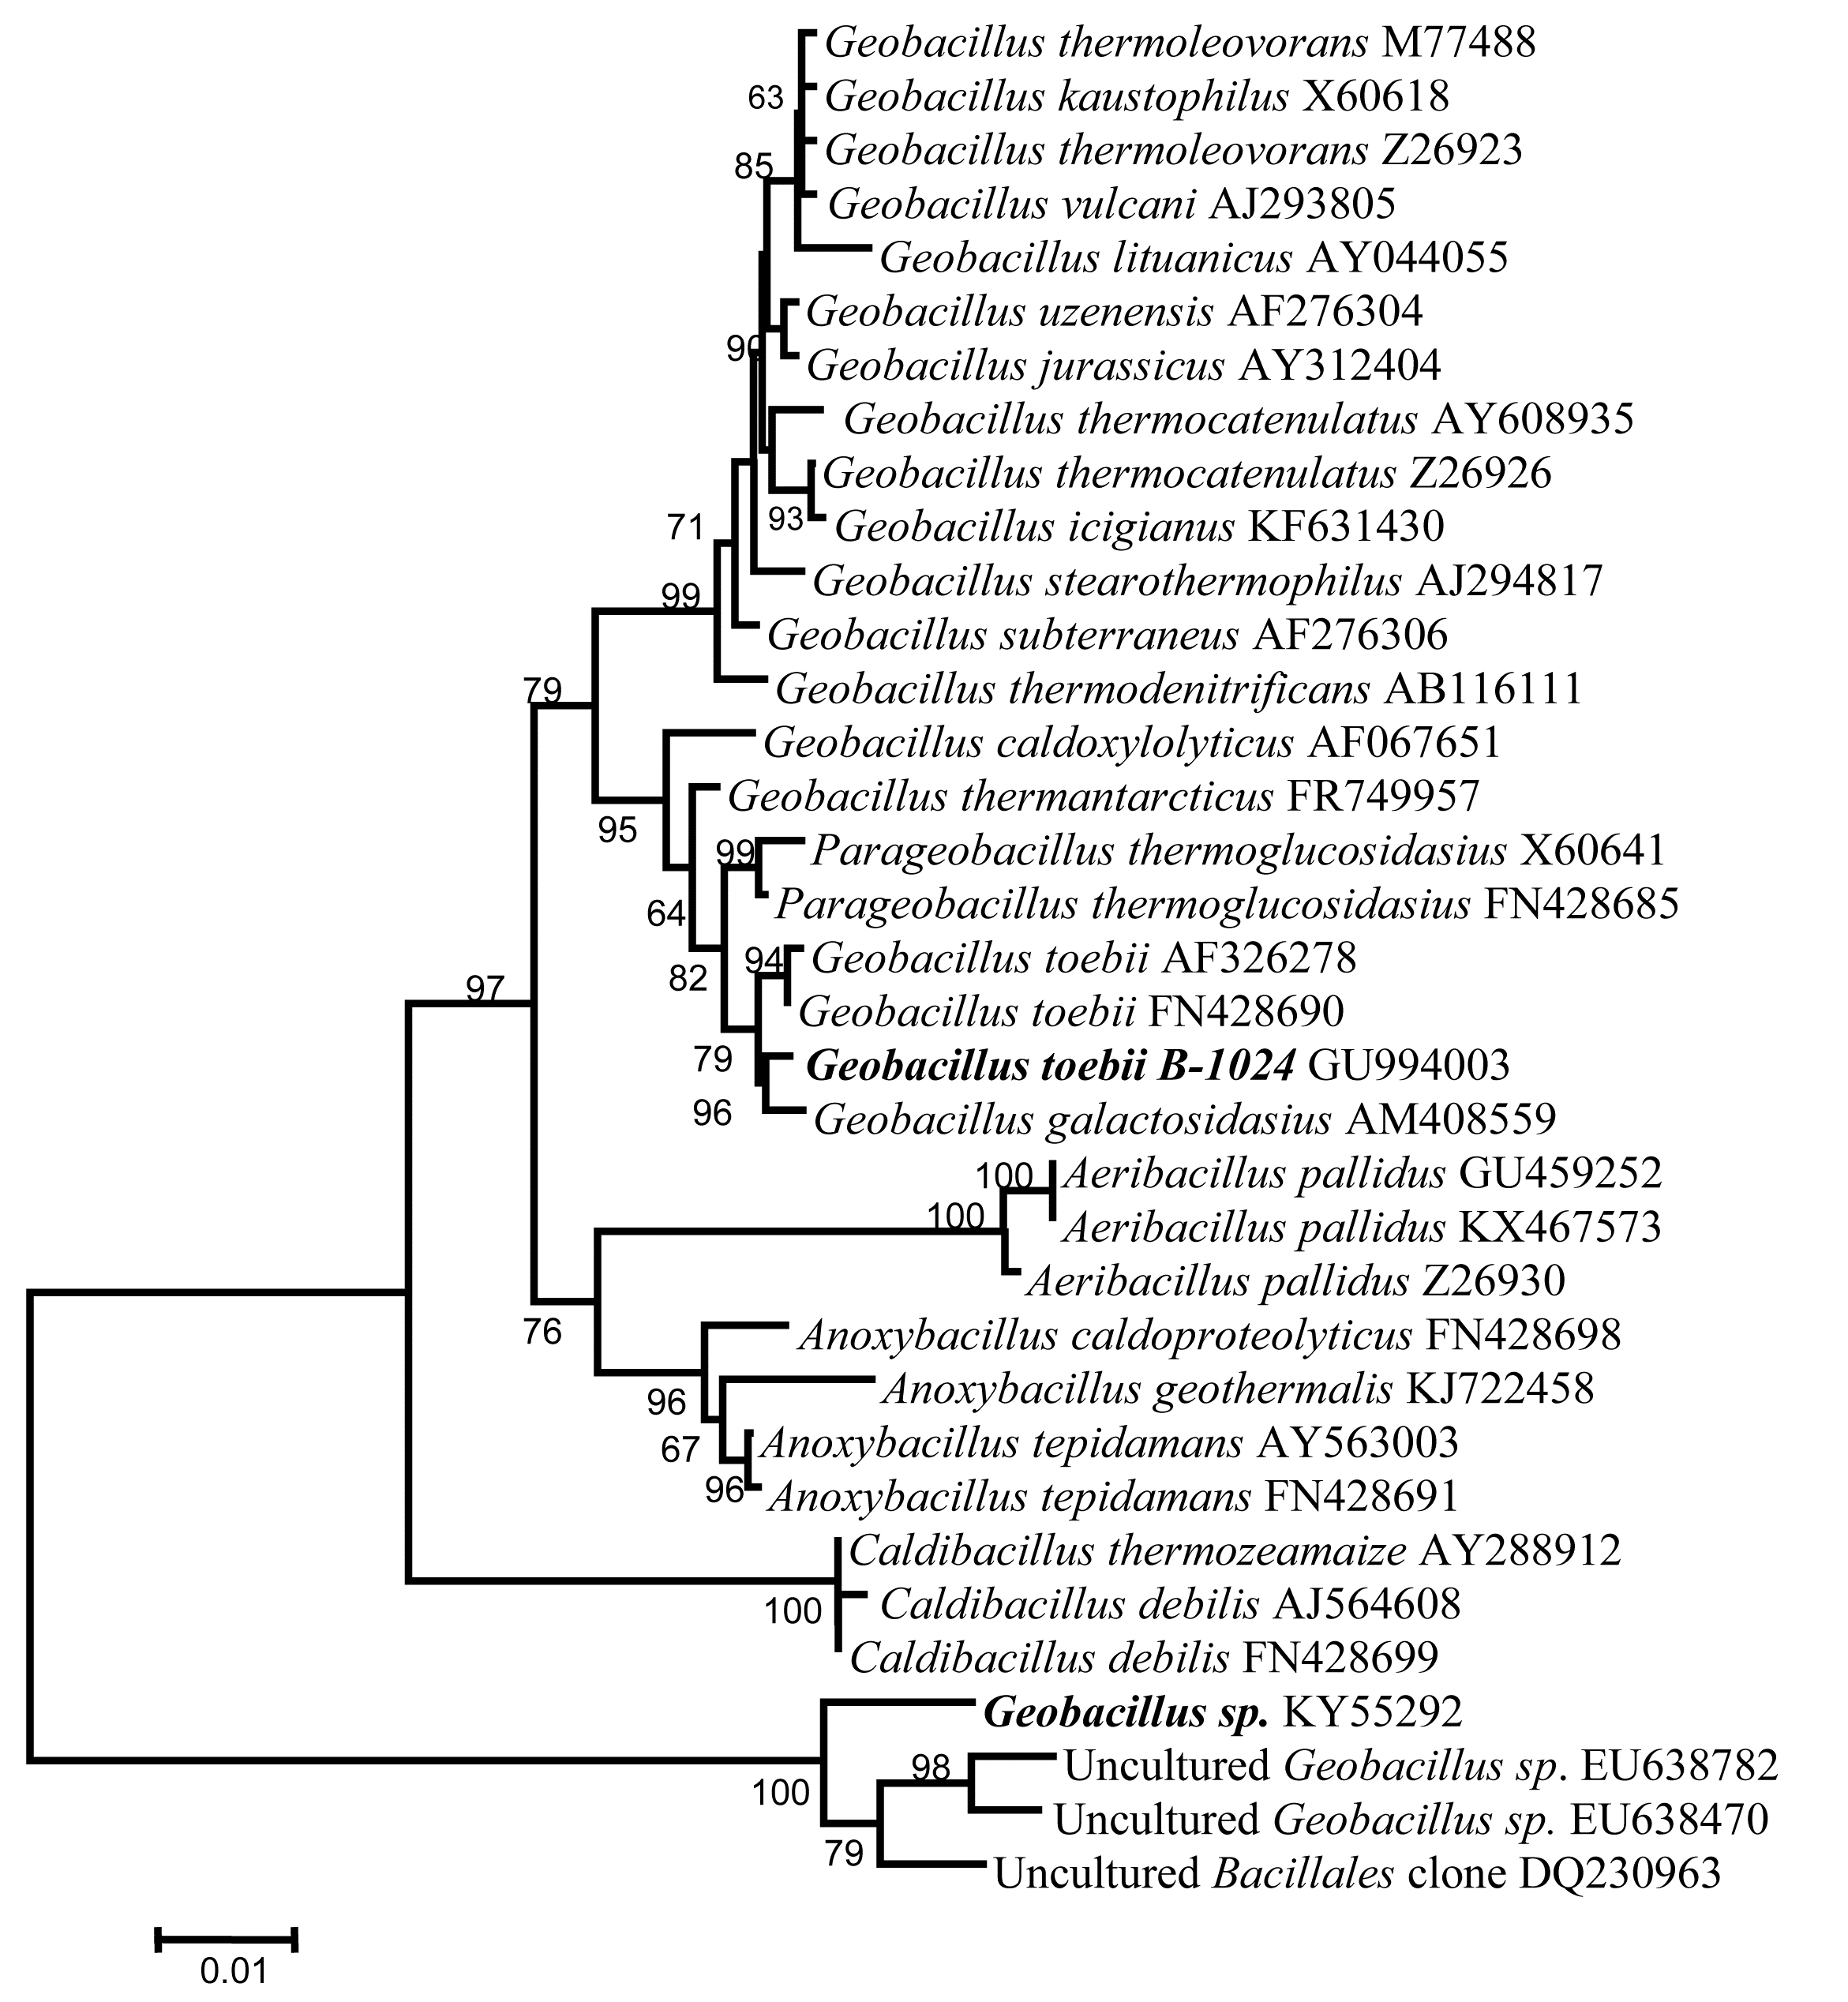
\includegraphics[width=0.9\linewidth]{media/image13.png}

\caption{Филогенетическое древо нуклеотидных последовательностей
гена 16S рРНК штамма \emph{Geobacillus} sp. и родственных
последовательностей рода \emph{Geobacillus}. Цифрами показана
достоверность ветвления, установленная с помощью ``bootstrap''- анализа
100 альтернативных деревьев; жирным шрифтом выделен штамм, исследованный
в данной работе и штамм В-1024, который был выделен из горячих
источников Байкальской рифтовой зоны (Tourova \textit{et al}., 2010).}\label{fig:5-2}
\end{figure}

Известно, что представители рода \emph{Geobacillus} обладают уникальными
гемицеллюлолитическими системами, что позволяет рассматривать их в
качестве потенциальных источников высокоактивных и термостабильных
ферментов для эффективного гидролиза биомассы. Данные микроорганизмы
также обладают высокой скоростью роста и способностью утилизировать
широкий круг субстратов, включая пентасахара (Brock \textit{et al}., 1978;
Bonch-Osmolovskaya, 2005; Rozanov \textit{et al}., 2013).

Полученные штаммы депонированы в открытый коллекционных фонд
Всероссийской коллекции микроорганизмов (ВКМ) (г. Пущино) с приложением
информации о культурах микроорганизмов в виде паспорта. Получены
Сертификаты о депонировании штаммов и их доступности. Штаммам
\emph{Geobacillus posolskii} PB15/Grf7geo и \emph{Thermaerobacter
baikalensis} PB12/4term присвоены номера VKM B-3150\textsuperscript{Т} и
VKM B-3151\textsuperscript{Т}, соответственно. Биомасса двух культур
\emph{Geobacillus posolskii} PB15/Grf7geo и \emph{Thermaerobacter
baikalensis} PB12/4term также бы ла направлена для депонирования в
немецкую коллекцию микроорганизмов и клеточных культур, г. Лейбниц,
Германия (DSMZ) после согласования всех необходимых процедур с куратором
Отдела Грам-положительных бактерий в Leibniz-Institute DSMZ. В настоящее
время, проводится работа по накоплению биомассы этого штамма для
повторной отправки в коллекцию.

\chapter{Среда поддержки научных исследований в секвенировании}\label{chap:5}\label{do:cherk}

Исследования по данному направлению направлены на решение проблемы
проектирования и реализации распределенной программной среды для
создания организационных, информационных и вычислительных ресурсов
проведения научных микробиологических исследований на основе
метагеномного анализа. Построена обобщенная модель предметной области
системного уровня и выделены требования к разрабатываемой среде, задачи,
требующие решения; построена и реализована модель вычислительного
процесса анализа ампликонов в виде графа управления вычислительным
процессом в среде Rapidminer. Разрабатываемая программная среда
позволит решать задачу построения информационного портала для обработки
метагеномных данных и представления результатов научному сообществу.

Для обеспечения~ метагеномных исследований требуются значительные
вычислительные ресурсы, а также участие квалифицированного
биоинформатика в обработке и интерпретации данных. Используемое в
научных исследованиях ЛИН СО РАН программное обеспечение анализа
ампликонов включает в себя различные библиотеки модулей обработки
последовательностей, например, Mothur, USearch, статистические пакеты и
среды разработки алгоритмов многомерного статистического анализа данных,
например, R
(\href{https://www.r-project.org/}{{https://www.r-project.org}}). Для
проведения исследований с использованием обработки и анализа
метагеномных данных специалисту требуются навыки составления сценариев в
командной оболочке операционной системы (Linux, Windows), запуска
пакетов в распределенной вычислительной среде и кластерных
вычислительных системах, а также программирования на языках общего
назначения, как правило, R или Python.

Существуют два основных вида метагеномных исследований. Первый, более
простой, называется анализом ампликонов. При этом амплифицируется и
секвенируется определённый таксономический маркер, универсальный для
исследуемых видов. Прочтения, полученные при секвенировании выделенной
из исследуемого образца ДНК, сравниваются с существующими базами данных,
что позволяет отнести их к тому или иному таксону разного
систематического уровня и получить информацию о разнообразии микробиоты
в исследуемой среде.

Вторая разновидность, известная как метагеномика методом «дробовика»
(shotgun metagenomics), основывается на секвенировании всей имеющейся в
пробе ДНК, а не конкретных локусов. При достаточном покрытии такой
подход позволяет описать не только таксономический состав сообщества, но
и присутствующие в геномах представителей сообщества гены функциональных
или структурных белков, в том числе -- вирусных. На основе метагеномных
данных устанавливаются метаболические взаимодействия в отдельных
микробиомах, опираясь на базы данных ePGDBs (environmental
pathway/genome databases). В некоторых работах из метагеномных наборов
прочтений удавалось выделить полные геномы отдельных видов.

Научным сообществом разработаны форматы данных для хранения метагеномной
информации, алгоритмы и программные модули, включая параллельные и
распределенные реализации на кластерных вычислительных системах,
обеспечивающие различные этапы анализа данных. Анализ предметной области
показал, что задачи, решаемые как в биоиформационной части метагеномного
анализа, так и в NGS в целом, хорошо представляются в рамках парадигмы
Больших Данных. Вычислительный процесс представляет собой, как правило,
последовательность запусков вычислительных утилит с передачей им
параметров в виде набора файлов. Вычислительный процесс представляет
собой сетевой граф элементарных операций, который строится на основе
передаваемой между модулями информации. Циклические структуры редки,
причем они, в основном, порождаются в результате анализа промежуточных
данных и результатов специалистами-предметниками: при
неудовлетворительном качестве тот или иной модуль перезапускается
человеком вручную с новыми параметрами.

Обработка Больших Данных требует от исследователя-предметника (биолога)
квалификации профессионального программиста-биоинформатика, так как
исследования каждой пробы требуют составления отдельной
программы-сценария или исполнения сценария вручную, что существенно
замедляет процесс получения конечного результата. Поэтому предложенная и
реализуемая концепция организации исследований базируется на создании
информационно-вычислительной среды, позволяющей проектировать и
воспроизводить сценарии, подавая на вход данные различных форматов из
различных источников, например, файлов, баз данных, серверов
метагеномной информации. В результате в среде строятся специальные
варианты вычислительных процессов, решающих задачи, поставленные
биологом. Необходимо также обеспечить также организованное облачного
хранения промежуточных данных и результатов. На этапе 2017 года в
проекте решалась задача исследования предметной области вычислительного
процесса и ее декомпозиция на классы задач (функциональное
моделирование). В результате такого моделирования выделены классы задач,
которые, затем, представлены в виде программных модулей. Из модулей
формируются сценарии решения задач, сетевые графы модулей, связанные
друг с другом передачей данных.

Популярным подходом к представлению вычислительного процесса, который
строится в виде комбинации исполняющих модулей, выступает
\emph{программирование потоков данных} (\emph{dataflow programming}).
Модули получают на вход некоторые данные, обрабатывают их и выдают на
выход. Результаты вычислений передаются на вход других модулей. Подход
развивается с 1970-х годов и имеет приложения в самых различных
областях. ~Подход удобен тем, что модули и сценарий их исполнения удобно
задавать при помощи визуального редактора. Пользователь выбирает нужный
модуль из набора модулей, добавляет его в рабочую область. Затем
необходимо сцепить входы и выходы модулей (порты), обеспечив таким
образом передачу информации. В результате должен получиться сетевой
граф, не содержащий циклов и имеющий, как правило, один вход и один
выход. Вход графа подаются данные, требующие обработки, на выход графа
выдается результат. На рисунке~\ref{fig:ampl-an} представлен пример (сценарий)
использования разрабатываемой в проекте системы управления
вычислительным процессом анализа ампликонов.~

\begin{figure}[htbp]\centering
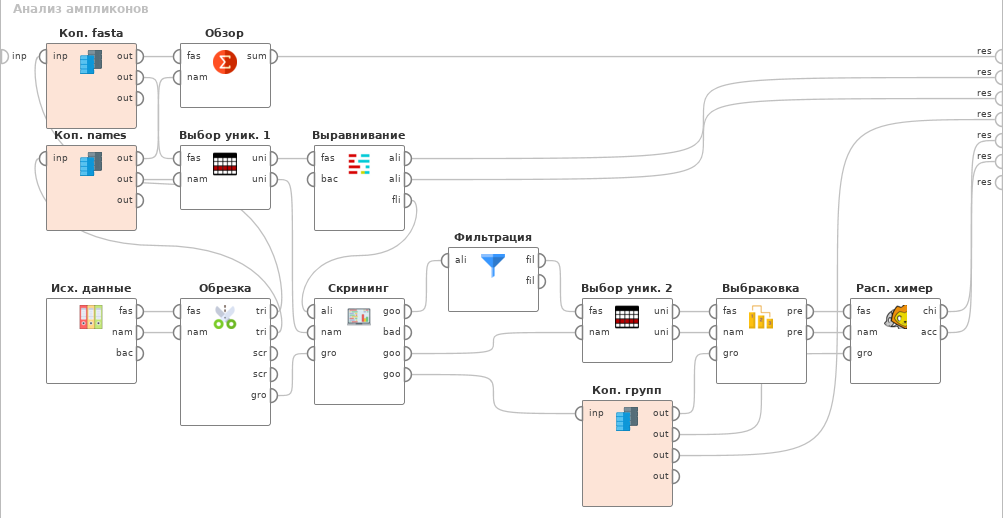
\includegraphics[width=0.9\linewidth]{media/image14.png}
\caption{Сетевой граф начальной стадии процесса анализа ампликонов}
\label{fig:ampl-an}
\end{figure}

Представленный сценарий сформирован при помощи программного комплекса
Rapidminer Studio (https://rapidminer.com/), дополненного в рамках
проекта разработанными модулями для представления этапов анализа
ампликонов. В сценарий входят следующие операции:

\begin{enumerate}
\def\labelenumi{\arabic{enumi}.}
\item
  формирование исследовательского проекта в виде папки (директории),
  содержащей данные секвенирования (модуль ``Исх. данные'');
\item
  обрезка данных (прочтений) (модуль ``Обрезка'');
\item
  модуль ``Обзор'' используется для визуального анализа качества
  результатов предыдущих шагов;
\item
  сокращение объема входных данных за счет удаления незначащей
  информации, например, дублирующих последовательностей (модули ``Выбор
  уник.'');
\item
  выравнивание последовательностей на референсные базы данных (модуль
  ``Выравнивание'');
\item
  фильтрация последовательностей по заданным критериям (модуль
  ``Скрининг'');
\item
  удаление колонок выравнивания по заданным критериям, например, пустых
  колонок (модуль ``Фильтрация'');
\item
  удаление последовательностей, содержащих ошибки секвенирования (модуль
  ``Выбраковка'');
\item
  обнаружение химер (модуль ``Расп. химер'', распознавание химер) и т.п.
\end{enumerate}

~В схеме представлены также сервисные модули Rapidminer, которые
необходимы для распространения однотипной информации между модулями
(``Коп. Групп'', копирование групп). Наличие таких модулей - это
особенность программной системы, предполагающей, что в общем случае
модули вносят изменения в обрабатываемую информацию без её копирования.

~Каждый модуль получает на вход название файла и в результате работы
создает новый файл. Функционирование модуля зависит от параметров,
задаваемых пользователем при помощи пользовательского интерфейса,
индивидуального для каждого модуля. Результаты работы сценария
передаются на специальные выходные порты и отображаются системой
Rapidminer Studio в удобном пользователю виде. Система поддерживает
возможность представления сценария в виде нового блока со своими портами
ввода и вывода, а также возможность облачного хранения и исполнения
сценариев, что позволяет создавать распределенные вычислительные среды.
Богатый набор функций Rapidminer, а также различные сервисы,
предоставляемые разработчиками стали основной причиной выбора этой
системы в качестве среды разработки информационно-вычислительных
ресурсов проекта.

Модули Rapidminer, отождествляемые с операциями NGS, разрабатываются на
языке программирования Java. Выбор этого языка обусловлен тем, что сам
редактор Rapidminer Studio реализован а системе программирования Java, а
стандартизированных интерфейсов к другим системам программирования
разработчиками еще не было сделано. В связи с этим процесс
программирования операции представляет собой

\begin{enumerate}
\def\labelenumi{\arabic{enumi}.}
\item
  Создание унаследованного класса, реализующего операцию: задание портов
  ввода и вывода, задание перечня параметров модуля, преобразование
  данных портов в вызов утилиты Motur, декодирование результатов работы
  программы, анализ ошибок времени исполнения Motur.
\item
  Описание интерфейса класса в виде XML-файла, читаемого редактором
  Rapidminer Studio.
\item
  Задание положения модуля в структуре модулей редактора.
\item
  Разработку пиктограммы операции, отображаемой внутри блока и
  символизирующей сущность операции.
\end{enumerate}

Дальнейшим направлением развития специализированной версии Rapidminer
является а) разработка системы интерпретации метаописаний операций
программы Mothur; б) реализация новых операций; в) интеграция с облачным
хранилищем (базой данных), разрабатываемым в рамках проекта; г) создание
интерфейса пользователя для специалистов-биологов, позволяющей им
самостоятельно проводить исследования и в некоторой степени влиять на
вычислительный процесс; д) разработка специализированных приложений и
библиотек операций, решающих специальные задачи.

Таким образом, для поддержки исследований в метагеномном анализе,
который позволяет описывать микробные сообщества с ранее недоступной
точностью, положено начало разработки средств автоматизации организации
исследований, направленных на обеспечение доступа к значительным
вычислительные мощностям и мощным алгоритмам анализа ампликонов
специалисту-биологу без значительного участия биоинформатиков. Данное
свойство системы обеспечивается при помощи визуального представления
операций, обобщением функций программного обеспечения и разработке
интерфейсов пользователя, ориентированных на специалистов-предметников.
В целом, разрабатываемая среда поддержки научных исследования позволит
предоставить исследователям удобный интерфейс анализа и обеспечить
хранение в унифицированной форме исходных данных и результатов анализа.

\chapter{Веб"=ориентированная информационная система управления данными результатов исследования микробиома озера Байкал}\label{chap:6}

С целью определения функциональных требований и проектирования
архитектуры веб-ориентированная информационная система управления
данными результатов исследования микробиома озера Байкал (ИС) проведен
анализ сложившейся практики в ЛИН СО РАН работы с данными в
исследованиях микробиома, охватывая следующие вопросы планирования и
исполнения рабочих процессов (вычислительных цепочек) обработки и
анализа метагеномных данных: используемое программное обеспечение,
объемы и скорость генерации данных, принятие решений, слабо
автоматизированные процессы (в которых активно используется «ручная»
обработка данных).

Также выполнен обзор известного программного обеспечения,
предназначенного для работы с данными в исследованиях микробиома в
рамках парадигмы Больших Данных. Выполнен сравнительный обзор наиболее
популярных современных платформ конвейерной обработки данных,
применяемых в научных исследованиях с интенсивным использованием данных,
в том числе, \textsc{Rapidminer}, \textsc{KNIME}, \textsc{Pipline Pilot},
\textsc{Taverna}. Сравнение произведено по таким характеристикам, как
модульность, требования к наличию навыков программирования у
исследователя, открытость исходного кода, интеграция с языком
программирования R, случаи применения в геномике и метагеномике.

В результате подготовлены предложения по включению известного
программного обеспечения в планируемый инструментарий, схем и форматов
данных, разработке инструментов планирования и исполнения вычислительных
технологических цепочек аналитики данных в исследовании микробиома оз.
Байкал, хранению и обработки больших объемов метагеномных данных в
распределенной среде на основе платформы \textsc{Hadoop}
(\href{https://hadoop.apache.org/}{{https://hadoop.apache.org}}).

Анализ сложившейся практики в ЛИН СО РАН показал, что для реализации
многоэтапных рабочих процессов обработки и анализа метагеномных данных
(pipline) вовлекаются различные программные комплексы обработки
последовательностей, статистические пакеты и скриптовые языки
программирования. Для исполнения таких цепочек приходится задействовать
высокопроизводительные вычислительные среды (суперкомпьютеры). Для
проведения таких исследований специалисту требуются навыки работы со
сценариями командной оболочки, запуска пакетов в распределенной
вычислительной среде, программирования на языках R или Python. Как
правило, для микробиологов реализация подобных цепочек вызывает
затруднения.

В настоящее время в ЛИН СО РАН для получения таблицы встречаемости
используется программный комплекс MOTHUR
(\href{https://www.mothur.org}{{https://www.mothur.org}}) с интерфейсом
командной строки. Некоторые этапы (например, кластеризация прочтений)
требовательны к вычислительным ресурсам. Их выполнение на локальной
рабочей машине пользователя занимает продолжительное время. Для решения
этой проблемы активно используются ресурсы Иркутского суперкомпьютерного
центра СО РАН (https://hpc.icc.ru). Цепочки обработки и анализа
метагеномных данных выполняются на вычислительном кластере «Академик
В.М. Матросов». Текущая реализация этого процесса сопряжена с рядом
сложностей: микробиологам ЛИН СО РАН приходится удаленно подключаться к
вычислительному кластеру по протоколу SSH (Secure Shell); каждая команда
вводится пользователем вручную в командной строке; хранение получаемых
данных не унифицировано, зависит полностью от пользователя, что
усложняет доступ к данным и их повторное использование другими
исследователями.

В рамках проекта разработан прототип веб-ориентированной информационной
системы управления данными результатов исследования микробиома озера
Байкал (ИС), направленная на преодоление перечисленных недостатков. ИС
преследует следующие цели: 1) управление данными (распределенное
хранение, обеспечение пользовательского и программного интерфейса
доступа) результатов исследования микробиома на протяжение их жизненного
цикла; 2) планирование и исполнение технологических цепочек обработки и
анализа больших объемов метагеномных данных.

\begin{figure}\centering
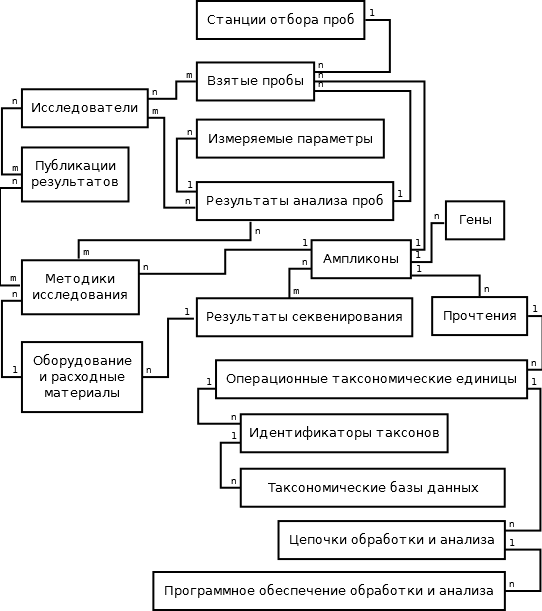
\includegraphics[width=0.9\linewidth]{media/image15.png}

\caption{Упрощенное представление схемы данных результатов
исследования микробиома, ребра, подписанные (1..n), соответствуют
отношениям типа один-ко-многим, подпись (n..m) показывает отношения типа
многие-ко-многим.}\label{fig:schemabd}
\end{figure}

Спроектирована схема хранения данных, получаемых при исследовании
микробиома озера Байкал (рисунок~\ref{fig:schemabd}). Схема охватывает информацию о сборе
проб, анализе физико-химических и биологических параметров этих проб,
результатов секвенирования, применяемом оборудовании, таксономических
базах, методиках анализа собранных материалов, публикациях результатов
исследований, а также исследователях, принимающих участие в получении
результатов. Также она позволяет хранить используемые вычислительные
цепочки обработки и анализа метагеномных данных, включая информацию о
программных инструментах, командах и конфигурационных файлов.

\begin{figure}\centering
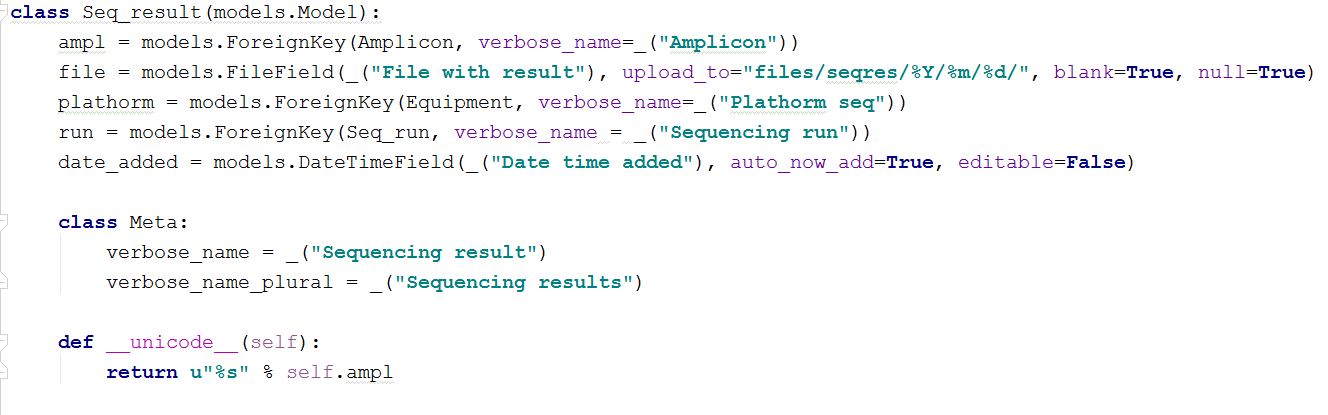
\includegraphics[width=0.9\linewidth]{media/image16.png}

\caption{Фрагмент модели ИС для инструментальной платформы \textsc{Django}}\label{fig:instrmod}

\end{figure}

На основе спроектированной схемы разработана информационная модель ИС,
обеспечивающая управление данных всего цикла исследования микробиома,
начиная от отбора пробы и заканчивая публикацией научных результатов.
Модель реализована средствами инструментальной платформы разработки
программного обеспечения \textsc{Django}
(\href{https://www.djangoproject.com}{{https://www.djangoproject.com}}).
Фрагмент модели представлен на рисунке~\ref{fig:instrmod}. По модели ИС создана
соответствующая структура базы данных в формате системы управления
данными \textsc{PostgreSQL}
(\href{https://www.postgresql.org}{{https://www.postgresql.org}}) и
сгенерирован настраиваемый пользовательский веб-интерфейс
административной панели, позволяющий на этапе разработки проводить
тестирование разработанной модели и тестовое наполнение базы данных
результатов исследования микробиома озера Байкал.

В текущей версии модели ИС реализованы следующие сущности данных:

\begin{itemize}
\item
  \emph{Организации} -- справочник научных организаций, проводящих
  исследования.
\item
  \emph{Исследователи} -- справочник исследователей с привязкой к
  аффилированным с ними организациям.
\item
  \emph{Водные объекты} -- справочник исследуемых водных объектов.
\item
  \emph{Зоны} -- справочник зон водных объектов (например, котловин
  озера Байкала) с привязкой к водным объектам.
\item
  \emph{Станции} -- пространственный список станций (мест отбора проб) с
  привязкой к водным объектам и их зонам.
\item
  \emph{Типы исследования} -- справочник типов исследования (физические,
  химические и др.).
\item
  \emph{Параметры} -- справочник физических, химических и других
  измеряемых параметров с привязкой к типам исследования.
\item
  \emph{Гены} -- список генов.
\item
  \emph{Публикации} -- список публикаций с результатами исследований, на
  которые могут ссылаться другие сущности с привязкой к исследователям,
  являющимися авторами данных публикаций.
\item
  \emph{Методы исследования} -- список методов, используемых в
  исследованиях с привязкой к используемому оборудованию и расходным
  материалам, а также публикациям с описанием данных методов.
\item
  \emph{Категории методов} -- поисковый справочник категориями методов
  исследования.
\item
  \emph{Программное обеспечение} -- список программных пакетов,
  используемых в рабочих процессах обработки и анализа метагеномных
  данных.
\item
  \emph{Таксономические базы данных} -- список баз данных, используемых
  для определения таксономических элементов.
\item
  \emph{Идентификаторы таксонов} -- список идентификаторов таксонов с
  привязкой к таксономическим базам данных.
\item
  \emph{Типы пробы} -- справочник типов пробы, (например, донные осадки,
  подлёдная проба, и др.).
\item
  \emph{Пробы} -- список отобранных проб с привязкой к станциям с
  привязкой к типам проб и станциям отбора проб.
\item
  \emph{Анализы проб} -- список результатов анализов проб по
  определённом параметрам (для одной пробы может быть проведено много
  разных анализов) с привязкой к собранным пробам, использованному
  оборудованию, расходным материалам и методам исследования, исследуемым
  параметрам, а также задействованным исследователям.
\item
  \emph{Типы оборудования} -- древовидный классификатор типов
  оборудования, используемого в исследовании.
\item
  \emph{Оборудование и расходные материалы} -- список оборудования и
  расходных материалов, используемых в исследовании (например, NGS
  платформы секвенирования), с привязкой к типам оборудования.
\item
  \emph{Рабочие процессы} -- список цепочек (pipeline) обработки и
  анализа метагеномных данных, обеспечивающий их воспроизведение, с
  привязкой к программному обеспечению.
\item
  \emph{Ампликоны} -- список ампликонов с привязкой к пробам, рабочим
  процессам, методам исследования и генам.
\item
  \emph{Запуски секвенирования} -- список выполненных запусков
  секвенирования с привязкой к исследователям и организациям.
\item
  \emph{Результаты секвенирования} -- список результатов секвенирования
  (файлов с данными секвенирования) с привязкой к запускам
  секвенирования, оборудованию и расходным материалам.
\item
  \emph{OTU} -- список полученных матриц OTU по результатам
  секвенирования с привязкой к рабочим процессам и идентификаторам
  таксонов.
\item
  \emph{Прочтения} -- список прочтений с привязкой к ампликонам и
  матрицам OTU.
\end{itemize}

Пользовательский веб-интерфейс доступа к данным разработанного прототипа
ИС настроен с использованием встроенных возможностей инструментальной
платформы \textsc{Django}. В пользовательском интерфейсе были
реализованы возможности добавления, редактирования и удаления для всех
представленных сущностей. Так же настроены элементы управления для
поиска, фильтрации, сортировки добавленных данных. Кроме того, при
добавлении данных пользователями перед отправкой данных на сервер,
осуществляется проверка вводимых данных, согласно заданным правилам, и в
случае ошибки ввода данных пользователь видит, где именно произошла
ошибка.

В настоящее время прототип ИС развернут в облачной вычислительной
инфраструктуре ИДСТУ СО РАН. Опытная версия ИС доступна по адресу
\href{http://ngs.icc.ru:88}{{http://ngs.icc.ru:88}}. Прототип развёрнут
в серверном дистрибутиве операционной системы \textsc{GNU/Linux CentOS}
версии 7.3. В качестве СУБД используется \textsc{PostgreSQL} версии 9.4,
а веб сервер сконфигурирован в связке инструментов
\textsc{nginx+gunicorn}. Такая реализация ИС позволила организовать
удаленный доступ к данным исследований микробиома, и в дальнейшем
позволит микробиологам самостоятельно управлять данными рабочих
процессов обработки и анализа метагеномных данных при исследовании
микробиома озера Байкал. В настоящее время начат тестовый ввод имеющихся
данных ЛИН СО РАН по исследованию микробиома озера Байкал.

\begin{figure}\centering
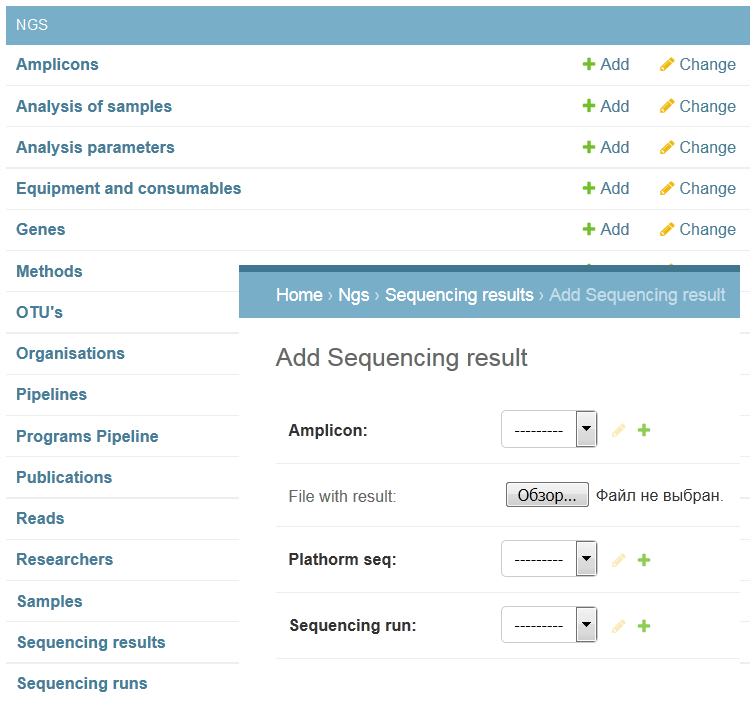
\includegraphics[width=0.9\linewidth]{media/image17.png}

\caption{Снимок экрана пользовательского веб-интерфейса опытной
версии ИС: форма доступа к данным результатов исследования микробиома
озера Байкал}
\end{figure}

\chapter{Заполнение хранилища больших данных}\label{chap:8}

Создана общая таблица с данными по станциям, их координатам, дате,
времени отбора проб, общей глубине станций, составу фитопланктона, общей
численности и биомассе фитопланктона, общей численности бактерий,
температуре, кроме того указаны маркерные гены, на основе которых
выполнено высокопроизводительное секвенирование, номера массивов данных
результатов высокопроизводительного секвенирования, загруженных в базу
данных NCBI Sequence Read Archive (SRA), а также методы выделения
суммарной ДНК и амплификации маркерных генов выполненных ранее в
2011-2013 г. На основе этих данных было проведено тестирование внесения
информации в Хранилище Больших Данных, сконструированное в ходе
выполнения данного проекта совместно с ИДСТУ СО РАН.

Создана коллекция суммарной ДНК и массивов информации, полученных ранее
в результате высокопроизводительного секвенирования, и служащих основой
для создания программно-аппаратной Инфраструктуры Обработки Больших
Данных (ИОБД). База данных включает следующую информацию: объект
исследования - водная толща или донные осадки; дата отбора проб; район
исследования, координаты; глубину водной толщи или донных осадков,
наименование библиотек генов, физико-химические параметры. Подготовлено
82 библиотеки генов 16S рРНК прокариот из районов разгрузки
газо-нефтесодержащих флюидов Южного и Среднего Байкала, естественных
выходов нефти у м. Горевой Утес и м. Толстый, грязевых вулканов
Маленький и Большой, низко-температурного источника в б. Фролиха,
метанового сипа Посольская банка, фоновых районов Южного Байкала и
Баргузинского залива. В базу данных параллельно вносится информация о
химическом составе поровых вод, данные по разнообразию (индексы Chao1 и
ACE), богатству (Shannon index и Simpson inverse index), количестве
полученных OTUs для каждого образца. Массивы последовательностей
депонированы в архив GenBank, секцию SRA, id: SRR3156030 (Bactеria) и
SRR3156034 (Archaea) для фонового района Южного Байкал; SRP045338,
SRR2912888 (Bactеria) и SRP052288, SRR2912890 (Archaea) для районов
разгрузок газо-нефтесодержащих флюидов.

Подготовлены данные о составе бактериальных сообществ (32 образца из
донных отложений и 26 образцов из водной толщи) и архейных сообществ (24
образца донных отложений). Часть образцов исследована с использованием
праймеров для двух регионов 16S рРНК: V2-V3 и V3-V4. Кроме того,
подготовлены 13 библиотек функциональных генов аэробного окисления
метана (\emph{pmoA}, \emph{mxaF}), и 13 библиотек генов 18S рРНК, а также последовательности сообществ из водной
толщи, подледных сообществ и др.

\chapter{Средства интеграции с мировой информационной средой}\label{chap:7}

Целью разработки данного направления является создание средств
интеграции результатов исследований в проекте с данными других
исследований, проводимых в России и за рубежом. Такая интеграция
позволит частично автоматизировать обработку информации, содержащейся в
материалах, первоначально предназначенных для ознакомления человеку,
например, отчетов, статей, страниц Интернет, баз данных и т.д.

Исследования велись по следующим направлениям:

\begin{enumerate}
\def\labelenumi{\arabic{enumi}.}
\item
  Поиск онтологий для представления публикуемых документов.
\item
  Разработка системы хранения и обеспечения публикуемых документов в
  частично формализованном виде.
\item
  Создание средств обеспечения доступа к документам, включая поиск по
  содержимому.
\item
  Разработка программной системы для построения логического вывода на
  данных документов.
\end{enumerate}

В основе концепции публикации данных является поддержка технологий
открытых связанных данных (Linked Open Data). Технологии позволяют
осуществлять интеграцию данных на уровне глобальных идентификаторов
ресурсов (URI, Universal Resource Identifiers) и общих стандартных
концептуальных моделей (онтологий), используемых для представления
данных (атрибутов и связей) публикуемых ресурсов.

Как правило, в процессе публикации ресурсов в Интернет решаются
следующие технические проблемы:

\begin{enumerate}
\def\labelenumi{\arabic{enumi}.}
\item
  Представление структуры публикуемых объектов при помощи стандартных
  форматов, позволяющих предоставлять доступ к имеющейся информации
  внешним ресурсам, алгоритмически обрабатывать публикуемую информацию.
\item
  Реализация серверов непосредственно предоставляющих требуемую
  информацию по запросу: по идентификатору или характеристике
  содержимого, например, по ключевым словам, тегам или части текста.
\item
  Создание средств обнаружения публикуемой информации: регистрация
  собственных ресурсов в известных системах поиска информации.
\end{enumerate}

На этапе исследований по проекту в 2017 году удалось продвинуться в
решении первых двух задач: изучен и проанализирован ряд стандартных
онтологий, используемых для публикации данных разного рода, в том числе
научных данных. Разработано программное обеспечение для
непосредственного предоставления ресурсов по запросу (цифровой архив),
поддерживающий несколько видов запросов (по содержимому, по адресу
ресурса и SPARQL). Цифровой архив снабжен средствами логического вывода
для поддержки решения задач связанных с предварительной обработкой
запрашиваемой информации на основе формализованных знаний. Процедуры
логической обработки также запускаются в результате соответствующего
типа запроса (Pengines), в результате чего порождаются новые табличные
данные -- качественные суждения о наборе объектов.

Основным публикуемым документом в проекте является научная статья.
Статья включает содержательную информацию, представляемую в виде текста,
таблиц, графиков и рисунков. На первом этапе рассмотрена и решена задача
структурной разметки документа, организацию документов в структуры
зависимостей по передаче информации. Полученные результаты позволяют
нацеливаться на решение задач разметки текста, представляющего
закономерности, логические и ассоциативные связи между объектами и
явлениями, реализуемых на следующих этапах.

Структурная разметка материалов публикаций использует следующие
онтологии:

\begin{enumerate}
\def\labelenumi{\arabic{enumi}.}
\item
  \href{http://www.openannotation.org/}{{Open Annotation}} (oa).
  Основная задача данной онтологии - представлять содержимое
  (аннотацию), описывающее другое содержимое. Закладка браузера является
  примером такого содержимого.
\item
  \href{http://xmlns.com/foaf/spec/}{{Friend-of-a-friend}} (foaf)
  позволяет представлять информацию об агентах: физических и юридических
  лицах, а также программных агентов.
\item
  \href{https://www.w3.org/TR/prov-o/}{{Provenance}} (prov). Онтология
  prov -- основа описания информационных потоков в документах и их
  взаимосвязи. В цифровом архиве prov используется для ассоциации
  документа с цифровым архивом и организацией владельцем.
\item
  \href{http://dublincore.org/documents/dcmi-terms/}{{Dublin Core}} (dc)
  представляет в аннотации ментаинформацию о творческом произведении:
  авторов, формат содержимого, его описание и др.
\item
  \href{http://wiki.dbpedia.org/}{{DBPedia}} resource (dbr) --
  пространство имен объектов (ресурсов) Wikipedia. Онтология dbr
  используется для обозначения конкретных сущностей, географических
  названий и т.п.
\item
  \href{http://bibliographic-ontology.org/specification}{{Bibliographic
  ontology}} (bibo) предназначена для разметки ссылок на внешние
  публикации, активно использует онтологию dc.
\item
  \href{http://schema.org/}{{Schema.org}} (schema) представляет объекты,
  распознаваемые поисковыми агентами Google, Yandex, Yahoo и др.
\end{enumerate}

Кроме перечисленных онтологий используются стандартные онтологии (RDF,
RDFs, RDFa, XSD) и онтологии из проекта
\href{https://userbase.kde.org/Nepomuk}{{NEPOMUK}}, предназначенные для
описания объектов, хранимых в полнотекстовых индексных цифровых архивах.

Предметная область NGS отражена в следующих онтологиях:

\begin{enumerate}
\def\labelenumi{\arabic{enumi}.}
\item
  \href{https://github.com/micheldumontier/semanticscience}{{Semanticscience
  Integrated Ontology}} (sio) задает простую интегрированную модель для
  объектов, процессов и их атрибутов. Онтология обеспечивает фундамент
  известных проектов по интеграции биологических данных
  \href{http://bio2rdf.org}{{Bio2RDF}} и
  \href{http://sadiframework.org}{{SADI}}
  (\href{http://sadiframework.org/content/about-sadi/}{{Semantic
  Automated Discovery and Integration}}).
\item
  \href{http://purl.org/biodiversity/taxon/}{{TaxonMap Ontology}}
  (taxon) - словарь для отображения таксономических классов в облако
  открытых связанных данных.
\item
  \href{http://purl.org/NET/biol/ns}{{Biological Taxonomy Vocabulary}}
  (biol) - словарь для представления таксономии всех форм жизни.
\item
  \href{http://www.biopax.org/}{{BioPAX Level 3 ontology}} (biopax) -
  онтология для представления процессов преобразования веществ и влияний
  (катализ, ингибирование и т.п.) веществ на биологические процессы. Она
  позволяет ученым обмениваться информацией друг с другом. Применение
  данной онтологии позволяет уменьшить сложность представления
  информации.
\item
  \href{http://biotopontology.github.io/}{{BioTop}} (biotop)
  используется для представления функциональных сущностей в биологии и
  медицине, представляет собой онтологию верхнего уровня, совместимую с
  онтологиями BFO, DOLCE, и UMLS Semantic Network.
\item
  \href{https://raw.githubusercontent.com/obi-ontology/obi/v2017-09-03/obi.owl}{{Ontology
  for Biomedical Investigation}} (obi) предназначена для разметки
  биомедицинские исследования, включая план исследования, протоколы и
  использованные приборы, а также позволяет представлять типы проводимых
  анализов и получаемые данные. Онтология obi получена
  усовершенствованием онтологии "Functional Genomics Investigation
  Ontology" (FuGO). Дальнейшее ее развитие направлено на включение
  концепций функциональной геномики и связанных с ней предметных
  областей.
\end{enumerate}

Популярным подходом к решению проблемы обнаружения данных является
регистрация сайтов/порталов в поисковых ресурсах, таких как Google или
Yandex. Данные информационные системы позволяют эффективно обнаруживать
ресурсы Интернета (конкретные статические и динамические страницы) по
ключевым словам и отрывкам текста. Для серверов, где все публикуемые
ресурсы (страницы) являются динамическими и генерируются во время
запроса их URI, данные сервера не предоставляют эффективной процедуры
обнаружения ресурсов по контексту, т.е. отображение свойств содержимого
на URI ресурса. Повышение эффективности обнаружения и предоставление
информации об общей структуре ресурса используются специализированные
средства, такие как Bio2RDF.

Проект Bio2RDF направлен разработку технологий обеспечения среды
связанных данных в науках о жизни. В основе разрабатываемых технологий
находится так называемый Семантический веб, программы и модули для
обработки соответствующим образом размеченной информации. Bio2RDF
определяет набор простых форматов данных и принципов их обработки,
создающих возможности
\href{https://docs.google.com/presentation/d/1SG6PFew2CPK1o_jRCYx30DFnuGEEr0uWVKPnz7Uqw5k/pub?start=false\&loop=false\&delayms=3000\&slide=id.p}{{интегрирования
данных из разных источников}}, представленных в различных форматах в
рамках технологий связанных данных. Действующий сервер, сопровождаемый
разработчиками, демонстрирует принципы Bio2RDF и семантические
технологии. Доступный исходный код позволяет свободно создавать
собственные ресурсы.

Сервисы Bio2RDF активно используют вышеперечисленные онтологии для
представления данных. Например, prov используется для указания источника
полученных данных. Сервер хранит ссылки на ресурсы источника данных в
виде отношений идентификаторов объектов в нотации ресурса и нотации
Bio2RDF. Кроме того, для всех объектов должен быть присвоен тип (класс).
Таким образом, сервисы Bio2RDF позволяют организовывать несколько
важнейших функций публикации данных -- обнаружение данных в результате
выполнения запросов на центральном сервере метаданных, обеспечение
ссылок на ресурсы в виде стандартных URL, что в свою очередь позволяет
загружать предоставленные данные и адаптировать их форматы к собственным
алгоритмам. Использование языка SPARQL на сервере метаданных позволяет
включать ресурсы сервера в комплексные запросы, задействующие несколько
серверов семантических данных. В результате запроса, как правило,
порождается ответ, похожий на реляционную таблицу. Такой подход и
обеспечивает интеграцию данных из разрозненных источников.

Публикация ресурсов осуществляется при помощи отображения URI ресурса на
его содержимое при помощи серверов, функционирующих по стандартному
протоколу HTTP. Реализация таких серверов обычно представляет собой
цифровой архив размеченных документов. В рамках проекта разработаны
архитектура и подсистемы такого цифрового архива, поддерживающего
технологии открытых связанных данных (рисунок
\href{file://///home/eugeneai/Development/text/Projects/Lin-2017/report-2017/annotation.html\#fig:architecture-LOD}{1}).

\begin{figure}\centering
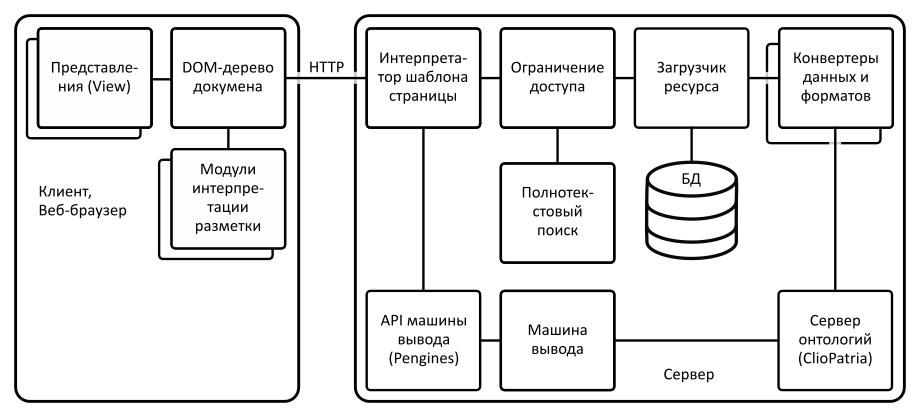
\includegraphics[width=0.8\linewidth]{media/image18.png}

\caption{Цифровой архив ресурсов проекта с обеспечением поддержки
  открытых связанных данных}
\end{figure}

Цифровые данные содержимого ресурсов хранятся в базе данных системы.
Система поддерживает множество таких баз данных. База данных
взаимодействует с загрузчиком данных, задача которого состоит в
преобразовании URI ресурса в содержимое. Для каждого источника
необходимо разрабатывать специальные конвертеры, задача которых состоит
в преобразовании публикуемой информации из базы данных в виде
содержимого, размеченного в соответствии с принципами открытых связанных
данных. В качестве форматов представления содержимого ресурсов выступают
размеченные RDFa HTML5-страницы или документы, а также графы онтологий,
представленные в TTL-, RDF- и OWL2-форматах.

Часть документов храниться в системе в ``разобранном'' виде и собирается
в веб-браузере в готовую статью. Модули интерпретации (порождения текста
документа) семантической разметки таких документов реализованы при
помощи клиентского JavaScript-интерпретатора, встроенного в веб-браузер.
Модули сканируют структуру дерева документа, распознавая условия их
активации. Если поиск оказался успешным, запускается тело модуля,
которое в общем случае вносит изменения в документ. Формирование
документа заканчивается, как только все условия были активированы и все
команды были обработаны.

Модуль разграничения доступа позволяет предоставлять доступ к данным на
основе некоторой политики, например, в соответствии с правами
зарегистрированного пользователя. Система позволяет загружать только те
ресурсы, т.е. получать доступ к URI ресурсов, соответствующие
полномочиям пользователя. Сервис полнотекстового поиска позволяет
ассоциировать тексты содержимого ресурсов с URI этих ресурсов.
Подсистема поиска реализована при помощи библиотеки Elasticsearch,
которая обладает средствами нечеткого сравнения термов, что позволяет
развивать систему в направлении реализации систем поиска релевантной
информации.

Интеграция с сервисами обнаружения ресурсов имеет несколько уровней
взаимодействия. На самом простом уровне сервер обнаружения лишь
предоставляет запрашивающей стороне только адреса URI зарегистрированных
ресурсов. Более тесная интеграция позволяет серверам выполнять
совместные (федеративные) запросы SPARQL. Для создания такой возможности
в цифровой архив добавлены блоки поддержки SPARQL, включая базу данных и
знаний (сервер онтологий), который используется для хранения
предварительно подготовленной логической структуры публикуемого ресурса.
Сервер онтологий реализован при помощи программной системы ClioPatria.
Данная система интересна тем, что полностью реализована на языках Prolog
и С, она предоставляет несколько форматов компактного хранения данных, а
также тесную интеграцию данных открытых связанных данных со средой
программирования языка Prolog.

Машина логического вывода языка программирования Prolog используется для
предварительной обработки публикуемой информации, а также для
обеспечения доступа к знаниям системы извне. Такой доступ обеспечивается
при помощи "API машины вывода" (Pengines). Данный интерфейс (API)
позволяет разрабатывать HTML5-JavaScript-приложения, отображающие тем
или иным способом данные из цифрового архива.

Благодаря использованию языка программирования Python и технологий
открытых связанных данных, а также модулей интерпретации разметки,
разработанный сервис публикации хорошо интегрируется с базами данных, в
том числе с разрабатываемой в рамках проекта базой данных научных
исследований.

Таким образом, на этапе 2017 года по данному направлению решены две
задачи -- разработан подход к описанию публикуемых данных при помощи
набора стандартных онтологий, разработан сервис публикации размеченных
документов, хорошо интегрирующийся с существующими цифровыми архивами и
базами данных.

\chapter{Моделирование динамики микробиома оз. Байкал}\label{chap:9}

В соответствии с основной целью проекта -- разработка математической
модели микробиома оз.Байкал -- на этапе 2017 года разработана процедура
идентификации структуры динамической модели взаимодействия организмов в
исследуемых сообществах альго-бактерий. Для поддержки исследований по
этому направлению спроектирован прототип программной системы,
организующий процесс исследований: предоставляется графический
пользовательский интерфейс для визуального отображения всех этапов
построения и расчета математической модели, результаты каждого этапа
моделирования представлены в виде соответствующих визуальных структур,
обеспечивается интеграция вычислительных подсистем в рамках одного
исследовательского приложения.

Различные виды организмов тесно связанны между собой различными
механизмами взаимодействия. В экосистеме озера Байкал большая часть
первичной продукции производиться фитопланктоном. Продуктивность
фитопланктона в свою очередь связанна с рядом внешних факторов
(температура, освещенность, концентрация биогенных элементов). Первичная
продукция, полученная в ходе фотосинтеза, утилизируется, в том числе и
бактериями, входящими в сложную систему альго-бактериальных
взаимодействий. Одним из путей прогнозирования поведения такой сложной
системы является ее представление в виде динамической модели,
позволяющей отслеживать эволюцию и поведение системы во времени.
Математическое моделирование системы осуществляется с применением
математического аппарата дифференциальных уравнений. Этап идентификации
модели микробиома проводится в три этапа. Первый этап - статический
корреляционный анализ имеющиеся информации по численности и биомассе
видов, входящих в состав сообщества, концентрации биогенных элементов в
воде озера. В результате корреляционного анализа определяются виды
взаимодействий в рамках сообщества, их численность, биомасса видов, а
также их связь с концентрациями биогенов в воде озера. Второй этап -
разработка концептуальной сети взаимодействия видов друг с другом и с
окружающей средой, представления сети взаимодействий в виде размеченного
графа. Третий этап - создание на основе этого графа системы специального
варианта системы дифференциальных уравнений, позволяющей прогнозировать
поведение системы с течением времени.

Для поиска попарных взаимосвязей между представленностью видов
бактериопланктона, в пробах; представленностью видов сообщества
микроорганизмов; биомассой исследуемых доминирующих видов диатомовых в
пробах; физико-химическими показателями воды (в число которых вошла
общая биомасса фитопланктона) был использован корреляционный анализ с
применением коэффициента корреляции Cпирмена \emph{r} (Hollander M.,
Wolfe D.A., 1973). Выбор способа расчета коэффициента корреляции основан
на предварительном анализе выборок с помощью критерия Шапио -- Уилка
(Patrick Royston 1995), который показал, что не все рассматриваемые
выборки представленности видов в пробах, выборки физико-химических
показателей воды в пробах и биомассы рассматриваемых видов диатомовых
водорослей распределены по нормальному закону. Все рассчитанные
коэффициенты корреляции объединены в корреляционную матрицу.
Корреляционная матрица визуализировалась с помощью \emph{тепловой карты}
полученной средствами пакета ``gplot'' (Gregory R. \textit{et al} 2015) языка
программирования R. Пакет ``gplot'' в данном случае использовался не
только для визуализации корреляционной матрицы, но и для параллельной
классификации показателей численности видов и физико-химических
характеристик среды по схожести коэффициентов корреляции, с помощью
кластерного анализа.

Проведен ряд расчетов по предложенной схеме идентификации. В качестве
примера анализа попарных взаимодействий приведем результаты
корреляционного анализа для определения связи между биотическим и
абиотическими показателями среды и представленностью (численность)
некоторых видов бактериопланктона, доминирующего в фотическом слое
пелагиали озера Байкал. Представленность (численность) видов
бактериопланктона оценивалась с помощью метагеномного анализа ампликонов
гена 16S рибосомальной РНК.

\begin{figure}\centering


\includegraphics[width=0.8\linewidth]{media/image19.jpeg}
\caption{Тепловая карта, отражающая корреляционную зависимость между
параметрами среды, в число которых входит общая биомасса фитопланктона с
численностью доминирующих в пробе видов бактерий. Виды бактерий отмечены
как OTU, каждый со своим номером.}\label{fig:heatmap-1}
\end{figure}

Анализ корреляции между бактериальными видами (OTU) и биомассой видов
фитопланктона показал, что OTU 40 и OTU 30 (\emph{Synechococcus})
отрицательно коррелируют с биомассой видов весеннего фитопланктона (рисунок~\ref{fig:heatmap-1}). Небольшое количество OTU положительно коррелировало с биомассой
видов фитопланктона. С биомассой \emph{S. acus} subsp. \emph{radians}
положительно коррелировало OTU 37 \emph{Cryomorphaceae} (r=0.47); с
\emph{A. baicalensis} -- OTU 89 \emph{Chitinophagaceae} (r=0.43), OTU 53
\emph{Actinomycetales} (r=0.38). С \emph{G. baicalense} положительно
коррелировали OTU 33, 19 (\emph{Ilumatobacter}), OTU 32, 155
(\emph{Verrucomicrobia} Subdivision3), OTU 81 Acidimicrobineae, OTU 127
Unclassified \emph{Bacteria}, и отрицательно коррелировали OTU,
принадлежащие \emph{Bacteroidetes} и \emph{Betaproteobacteria} (рисунок~\ref{fig:heatmap-1}).

Кластерный анализ, проведенный на основе сходства спектров коэффициентов корреляций для различных показателей на тепловой карте, позволяет выявить группы бактерий со схожей реакцией на биотическое и абиотическое воздействие. На основе кластерного анализа в примере, представленном на рисунке \ref{fig:heatmap-1}, выделены две группы видов микроорганизмов. Первая группа видов имеет положительные коэффициенты корреляции с температурой и концентрацией биогенов в воде и отрицательные коэффициенты корреляции с общей численность бактерий, биомассой фитопланктона, кислотность среды и концентрацией кислорода. Вторая группа объединяет виды бактерий, которые попадают в одеяльный кластер. Виды бактерий второй группы не имеют четких закономерностей по распределению значений коэффициентов корреляций.

Динамическая модель включает, в простейшем случае, следующие характерные компоненты альго"=бактериального сообщества: 1) меняющаяся во времени концентрация растворенных биогенов воде, обозначаемая r\textsubscript{1}; 2) меняющаяся во времени численность какого либо вида фитопланктона h\textsubscript{1}; 3) масса первичного органического вещества m; численность определенного вида фитопланктона, потребителя первичного органического вещества b\textsubscript{1}. Количество компонентов в системе определяется количеством взаимодействующих видов и количеством первичных ресурсов, доступных для этих видов. В общем виде рассмотренная четырехкомпонентная система описывается уравнением~(\ref{eq:four-comp-sys}).

\begin{equation}
\left\{ \begin{array}{lcl}
\frac{dr_{1}}{\text{dt}} &=& c\left( t \right) - p_{1}h_{1} - z_{1}b_{1},\\
\frac{dh_{1}}{\text{dt}} &=& a_{1}h_{1} - \frac{s_{1}h_{1}^{2}}{r_{1}},\\
\frac{\text{dm}}{\text{dt}} &=& \frac{s_{1}h_{1}^{2}}{r_{1}},\\
\frac{db_{1}}{\text{dt}} &=& v_{1}b_{1} - \frac{k_{1}b_{1}^{2}}{mr_{1}}.
\end{array} \right. \label{eq:four-comp-sys}
\end{equation}

В этом уравнении параметры имеют следующий биологический смысл: \(c(t)\) --
приток биогена в озеро, \(p_{1}\) -- скорость элиминации биогена из
окружающей среды фитопланктоном, \(z_{1}\) -- скорость элиминации
биогена из окружающей среды бактериопланктоно, \(a_{1}\) - скорость
размножения фитопланктона, \(s_{1}\) -- коэффициент, определяющий
интенсивность вымирания фитопланктона в единицу времени из-за
конкуренции за общие ресурсы, \(v_1\)- скорость размножения бактериопланктона и
\(k_{1}\) -- коэффициент, определяющий интенсивность вымирания
бактериопланктона в единицу времени из-за конкуренции за общие ресурсы.
В уравнении фигурирует кадратичная смертность из-за конкуренции за общие
ресурсы и рождаемость по экспонециальному закону.

В случае если в системе фигурирует \emph{n} видов первичного ресурса
(биогенов), \emph{l} видов фитопланктона и \emph{d} видов
бактериопланктона, то система уравнений~(\ref{eq:four-comp-sys}) примет вид~(\ref{eq:four-comp-sys-spec}).

\begin{equation}
 \left\{ \begin{array}{lcl}
\frac{dr_{i}}{\text{dt}} &=& c_{i}\left( t \right) - \sum_{i}^{l}{p_{i}h_{i}} - \sum_{i}^{d}{z_{i}b_{i}},\\
\frac{dh_{i}}{\text{dt}} &=& a_{i}h_{i} - \frac{s_{i}h_{i}^{2} + \sum_{j}^{l}{w_{j}h_{j} + \sum_{j}^{d}{u_{j}b_{j}}}}{\prod_{i}^{n}r_{i}},\\
\frac{\text{dm}}{\text{dt}} &=& \sum_{i}^{l}\frac{s_{i}h_{i}^{2} + \sum_{j}^{l}{w_{j}h_{j} + \sum_{j}^{d}{u_{j}b_{j}}}}{\prod_{i}^{n}r_{i}},\\
\frac{db_{i}}{\text{dt}} &=& v_{i}b_{i} - \frac{k_{i}b_{i}^{2} + \sum_{j}^{d}{g_{j}b_{j} + \sum_{j}^{l}{z_{j}h_{j}}}}{m}.\\
\end{array} \right.
  \label{eq:four-comp-sys-spec}
\end{equation}

В данном уравнении параметры имеют тот же биологический смысл, что и в
предыдущей системе. Произошло добавление следующих параметров: \(w_{j}\)
-- параметр, определяющий интенсивность взаимодействия между
соответствующими видами фитопланктона; \(u_{j}\) -- параметр,
определяющий интенсивность взаимодействия между соответствующими видам
фитопланктона и бактерипланктона; \(g_{j}\) -- параметр, определяющий
интенсивность взаимодействия между соответствующими видами
бактерипланктона; \(z_{j}\) -- параметр, определяющий интенсивность
взаимодействия между соответствующими видам бактерипланктона и
фитопланктона. Значения \(w_{j}\), \(u_{j}\), \(g_{j}\), \(z_{j}\) равны 0, если
нет соответствующей корреляционной связи, больше 0, если связь
положительна, и меньше 0, если связь отрицательна.

Разрабатываемые модели визуализируются в виде графов взаимодействий
(рисунок~\ref{fig:graph}). Для построения таких графов их тепловых карт разработано
программное обеспечение для поддержки научных исследований Model Studio.
Тепловая карта анализируется по видам бактерипланктона и на первом этапе
представители видов распределяются по классам и близким OTU. Аналогично
распределяются взаимодействия. Подобное представление отображает
естественную структуру взаимодействия составляющих динамической модели
близкую к полисистемному расслоению.

Каждый слой полисистемы содержит объекты и взаимодействия,
характеризующиеся общими свойствами. В данном случае выделены четыре
слоя: внешние факторы (солнечная радиация, поступление углекислого
газа): водоросли, рост которых в основном определяется внешними
факторами; бактерии, численность которых зависит в основном от
жизнедеятельности водорослей; состояние водной среды, оказывающей
воздействие на слои водорослей и бактерий.

\begin{figure}\centering
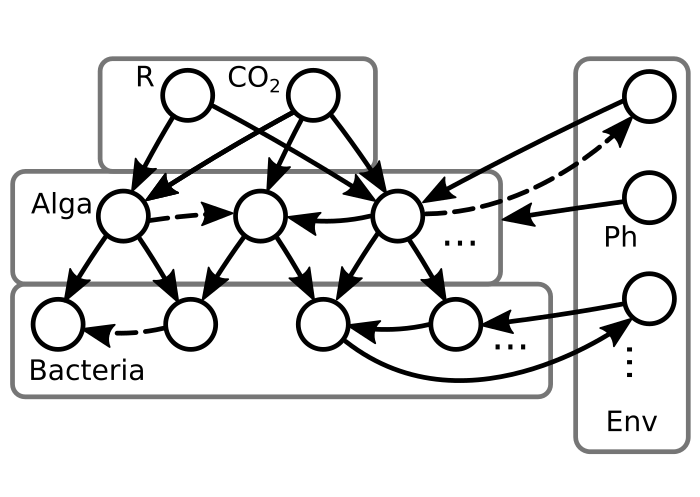
\includegraphics[width=0.4\linewidth]{media/image20.png}

\caption{Результат визуализации графа взаимодействий (пример)}\label{fig:graph}
\end{figure}

В программе Model Studio реализуются модули для представления
динамической модели сообществ в виде а) тепловой карты (рисунок~\ref{fig:heatmap-1}) б)
общего графа (рисунок~\ref{fig:graph}), в) графа data flow, аналогичного представлению
вычислительного процесса в Rapidminer, г) дифференциального уравнения,
д) перечня анализируемых критериев модели, е) результатов моделирования.
На рисунке~\ref{fig:heatmap} приведен пример интерфейса программы, отображающий тепловую
карту.

\begin{figure}\centering

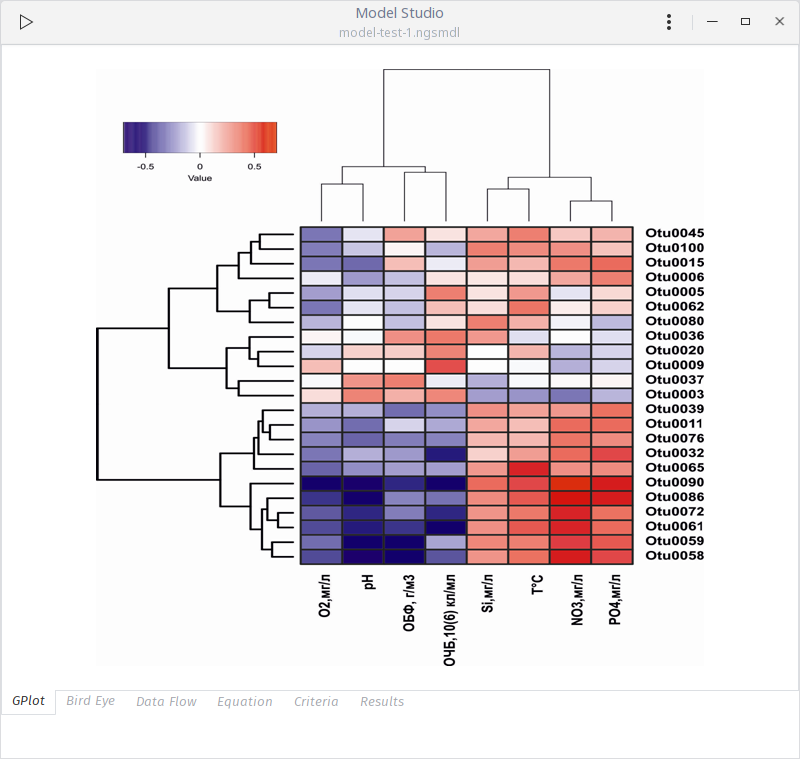
\includegraphics[width=0.9\linewidth]{media/image21.png}

\caption{Представление тепловой карты в Model Studio}\label{fig:heatmap}
\end{figure}

Model Studio реализуется при помощи ряда систем программирования:

\begin{enumerate}
\def\labelenumi{\arabic{enumi}.}
\item
  Python позволяет эффективно разрабатывать комплексные системы
  (склеивать компоненты) из различных гетерогенных подсистем, а также
  выступать в качестве удобного языка программного управления
  приложением; кроме того, использование этого языка позволяет в
  дельнейшем обеспечить взаимодействие с разрабатываемым в проекте
  хранилищем данных;
\item
  R для проведения этапа интеллектуального анализа данных, в этой среде
  реализованы процедуры анализа результатов секвенирования проб и
  построения корреляционных диаграмм;
\item
  Библиотека matplotlib, позволяющая строить графики и диаграммы и
  встраивать их в интерфейс пользователя, а также проводить экспорт в
  форматы, используемые в публикации данных;
\item
  SWI Prolog использована для формализации знаний этапа анализа
  структуры тепловой диаграммы и построения графа, а также для задания
  качественных критериев оценки результатов модели;
\item
  Библиотеки graphviz, использованной для раскладки графа на плоскости в
  процессе построения его визуального представления, кроме этой
  библиотеки для задачи визуализации задействованы библиотеки
  python-igraph, позволяющей обрабатывать большие по объему графы,
  NetworkX, предназначенной для изучения структур динамических сетей в
  биологии, социуме и технике, и graph-tool, поддерживающая многоядерные
  вычислительные архитектуры, фильтрацию данных, стандартные форматы
  данных, оценку статистических параметров графов, топологические
  алгоритмы, а также, в некоторой степени, возможности логического
  вывода на статических данных;
\item
  Языка Vala, подобный Java/С++/С\#, использован для реализации
  основного окна приложения и вычислительных процедур, язык представляет
  возможность разработки вычислительных процедур, т.к. в отличие от
  своих прототипов является компилируемым;
\item
  Среда разработки интерфейсов пользователя GTK+, которая позволяет
  интегрировать подсистемы приложения на уровне пользовательского
  интерфейса, а также разрабатывать кросс-платформенные приложения.
\end{enumerate}

Таким образом, на первом этапе проекта разработана первая версия
системы, интегрирующей различное программное обеспечение в рамках одного
приложения. Реализован ряд функций визуализации промежуточных данных и
результатов. Полученные результаты позволяют перейти к разработке
подсистем, обеспечивающих исследователя возможностью проведения
экспериментов с разрабатываемыми моделями, т.е. задачам следующего года
исследований. Разработанные алгоритмы опробованы на задачах, носящий
технический характер, т.е. направленных на тестирование алгоритмов и
систем приложения.

\chapter*{ЗАКЛЮЧЕНИЕ}
\label{chap:concl}

% Заключение должно содержать:
% - краткие выводы по результатам НИР в целом;
% - оценку полноты решений поставленных задач по НИР в целом;
% - рекомендации по конкретному использованию результатов НИР по НИР в целом;
% - оценку научного уровня выполненной НИР в целом в сравнении с лучшими достижениями в данной области.



... про данные и методологию их сбора

С целью поддержки процесса исследований начата разработка программных технологий автоматизации процесса хранения информации и обеспечения к ней эффективного интегрированного централизованного доступа на различных этапах анализа данных.  Разрабатываемые ресурсы соответствуют современным технологиям облачного хранения данных.  Существующие модели процессов обработки и анализа данных натурных исследований и экспериментов проанализированы, и разработаны соответствующие модели информационных потоков.  Полученные модели представляются в виде визуальных образов, позволяющих исследователям"=предметникам участвовать в проектировании процедур обработки, анализа и интерпретации данных и результатов.

Таким образом, результаты, полученные в проекте в \theyear{} представляют собой реализацию современной метеорологии исследований водоемов, широко используемых в мировой практике проведения научных исследований, но примененных к новому объекту исследования -- оз.~Байкал.  Полученные результаты носят мультидисциплинарный характер и на этапе \theyear{} года охватывают стадии сбора, обработки информации, а также совершенствование методов анализа полученной информации.

\appendices
%\appendix
%\appendixpage
%\addappheadtotoc

\begingroup
%\titleformat*{\chapter}{\relax}
%\titleformat*{\chapter}{\normalfont}
\begin{thebibliography}{99}
\bibitem{}
  Patrick Royston (1995) Remark AS R94: A remark on Algorithm AS 181:
  The \emph{W} test for normality. \emph{Applied Statistics},
  \textbf{44}, 547--551.
\bibitem{}
  Gregory R. Warnes, Ben Bolker, Lodewijk Bonebakker, Robert Gentleman,
  Wolfgang Huber Andy Liaw, Thomas Lumley, Martin Maechler, Arni
  Magnusson, Steffen Moeller, Marc Schwartz and Bill Venables (2015).
  gplots: Various R Programming Tools for Plotting Data. R package
  version 2.17.0.
  \href{http://CRAN.R-project.org/package=gplots}{{http://CRAN.R-project.org/package=gplots}}
\bibitem{}
  Hollander M., Wolfe D.A. (1973), \emph{Nonparametric Statistical
  Methods.} : John Wiley \& Sons. Pages 185--194 (Kendall and Spearman
  tests).
\bibitem{}
  Karsenti \textit{et al}. A Holistic Approach to Marine Eco-Systems Biology //
  PLoS Biol. 2011. Vol. 9. № 10. P. e1001177;
\bibitem{}
  Karsenti Towards an `Oceans Systems Biology' // Mol. Syst. Biol. 2012.
  Vol. 8. P. 575

\bibitem{}
Allen L.Z., Allen E.E., Badger J.B., McCrow J.P., Paulsen I.T., Elbourne
L.DH., Thiagarajan M., Rusch D.B., Nealson ЛюРюб Williamson S., Venter
J.C., Allen A.E. Influence of nutrients and currents on the genomic
composition of microbes across an upwelling mosaic //
\href{https://www.ncbi.nlm.nih.gov/pmc/articles/PMC3379637/}{ISME J}.
2012; 6(7): 1403--1414.
doi:~~\href{https://dx.doi.org/10.1038\%2Fismej.2011.201}{10.1038/ismej.2011.201}.

\bibitem{}
Fouhy F., Clooney A.G., Starton C., Claesson M., Cotter P.D. 16S rRNA
gene sequencing of mock microbial populations- impact of DNA extraction
method, primer choice and sequencing platform //
\href{https://www.ncbi.nlm.nih.gov/pmc/articles/PMC4921037/}{BMC
Microbiol}. 2016; 16: 123.doi:
\href{https://dx.doi.org/10.1186\%2Fs12866-016-0738-z}{10.1186/s12866-016-0738-z}.

\bibitem{}
Gerasimidis K., Bertz M., Quince C., Brunner K., Bruce A., Combet E.,
Calus S., Loman N., Jiaz U.Z. The effect of DNA extraction methodology
on gut microbiota research applications //
\href{https://www.ncbi.nlm.nih.gov/pmc/articles/PMC4960752/}{BMC Res
Notes}. 2016; 9:
365.doi:~~\href{https://dx.doi.org/10.1186\%2Fs13104-016-2171-7}{10.1186/s13104-016-2171-7}.

\bibitem{}
Rusch D.B., Halpern A.L., Sutton G., Haidelberg K.B., Williamson S.,
Yooseph S., Yooseph S., Wu D., Eisen J.A., Hoffman J.M., Remington K.,
Beeson K., Tran B., Smith H. The~\emph{Sorcerer II}~Global Ocean
Sampling Expedition: Northwest Atlantic through Eastern Tropical Pacific
// Plos Biology, 2007,
\url{https://doi.org/10.1371/journal.pbio.0050077}

\bibitem{}
Smith M.W., Allen L.Z., Allen A. E., Simon H.M., Contrasting genomic
properties of free-living and particle-attached microbial assemblages
within a coastal ecosystem // Front. Microbiol.,
\url{https://doi.org/10.3389/fmicb.2013.00120}.

\bibitem{}
Wen Y., Xiao F., Wang C.,Wang Z. The impact of different methods of DNA
extraction on microbial community measures of BALF samples based on
metagenomic data //
\href{https://www.ncbi.nlm.nih.gov/pmc/articles/PMC4858570/}{Am J Transl
Res}. 2016; 8(3): 1412--1425.

\bibitem{}
\protect\hypertarget{h1}{}{}Шубенкова О.В., Земская Т.И., Черницына
С.М., Хлыстов О.М., Трибой Т.И. Первые результаты исследования
филогенетического разнообразия микроорганизмов осадков южного Байкала в
районе поверхностного залегания гидратов метана // Микробология. 2005.
Т.74. № 3. С. 370-377.

\bibitem{}
  Шубенкова О.В., Земская Т.И., Черницына С.М., Хлыстов О.М., Трибой
  Т.И. Первые результаты исследования филогенетического разнообразия
  микроорганизмов осадков Южного Байкала в районе приповерхностного
  залегания гидратов метана // Микробиология. 2005. Т. 74. № 3.С.
  370--377.
\bibitem{}
  Детекция генов деградации н-алканов \emph{alkB} и \emph{ladA} у
  термофильных углеводородокисляющих бактерий родов \emph{Aeribacillus}
  и \emph{Geobacillus} {[}Текст{]} / Т. П. Турова {[}и др.{]}
  //Микробиология. -- 2016. -- Т. 85. -- № 6. -- С. 679--692.
\bibitem{}
  Brock, T.D. (1978). Thermophilic microoganisms and life at high
  temperatures. US: Springer-Verlag.
\bibitem{}
  Bonch-Osmolovskaya, E.A. (2005). Phylogenetic and metabolic diversity
  of thermophilic prokaryotes with different types of anaerobic
  respiration. Microbial diversity: current perspectives and potential
  application. : International Publishing House.
\bibitem{}
  Rozanov, A.S., Ivanisenko, T.V., Bryanskaya, A.V., Shekhovtsov, S.V.,
  Logacheva, M.D., Saik, O.V., Malup, T.K., Demenkov, P.S.,
  Goryachkovskaya, T.N., Ivanisenko, V.A., Peltek, S.E. (2014).
  Bioinformatic analysis of the genome of the Geobacillus
  stearothermophilus 22 strain isolated from the Garga , Baikal region.
  Russian J. Genetics: Applied Research, 4, 267--272.
\bibitem{}
  Giovannoni SJ, Thrash JC, Temperton B. 2014. Implications of
  streamlining theory for microbial ecology. The ISME journal 8:1553.
\bibitem{}
  Morris RM, Rappé MS, Connon SA, Vergin KL. 2002. SAR11 clade dominates
  ocean surface bacterioplankton communities. Nature 420:806
\bibitem{}
  Daims H, Lebedeva EV, Pjevac P, Han P, Herbold C, Albertsen M,
  Jehmlich N, Palatinszky M, Vierheilig J, Bulaev A. 2015. Complete
  nitrification by Nitrospira bacteria. Nature 528:504.
\bibitem{}
  Weiss R, Carmack E, Koropalov V. 1991. Deep-water renewal and
  biological production in . Nature 349:665.
\bibitem{}
  Zeng Y, Feng F, Medová H, Dean J, Koblížek M. 2014. Functional type 2
  photosynthetic reaction centers found in the rare bacterial phylum
  Gemmatimonadetes. Proceedings 884 of the of Sciences 111:7795-7800.
\bibitem{}
  Hugerth LW, Larsson J, Alneberg J, Lindh MV, Legrand C, Pinhassi J,
  Andersson AF. 2015. Metagenome-assembled genomes uncover a global
  brackish microbiome. Genome biology 16:1-18.
\bibitem{}
  Mehrshad M, Amoozegar MA, Ghai R, Fazeli SAS, Rodriguez-Valera F.
  2016. Genome reconstruction from metagenomic datasets reveals novel
  microbes in the brackish waters of the Caspian Sea. Applied and
  environmental microbiology:AEM. 03381-15.

\bibitem{}
Petrosino, J. F., Highlander, S., Luna, R. A., Gibbs, R. A., Versalovic,
J.\emph{.} Metagenomic pyrosequencing and microbial identification
//Clinical chemistry. -- 2009. -- Т. 55. -- №. 5. -- С. 856-866.

\bibitem{}
Kim, M., Lee, K. H., Yoon, S. W., Kim, B. S., Chun, J., Yi, H. (2013).
Analytical tools and databases for metagenomics in the next-generation
sequencing era. \emph{Genomics \& informatics}, \emph{11}(3), 102-113.

\bibitem{}
Quail, M. A., Smith, M., Coupland, P., Otto, T. D., Harris, S. R.,
Connor, T. R., ... \& Gu, Y (2012)\emph{.} A tale of three next
generation sequencing platforms: comparison of Ion Torrent, Pacific
Biosciences and Illumina MiSeq sequencers //BMC genomics. -- 2012. -- Т.
13. -- №. 1. -- С. 341.

\bibitem{}
Magoč, T., \& Salzberg, S. L. (2011). FLASH: fast length adjustment of
short reads to improve genome assemblies. \emph{Bioinformatics},
\emph{27}(21), 2957-2963.

\bibitem{}
Fosso, B., Santamaria, M., Marzano, M., Alonso-Alemany, D., Valiente,
G., Donvito, G., ... \& Pesole, G. (2015). BioMaS: a modular pipeline
for Bioinformatic analysis of Metagenomic AmpliconS. \emph{BMC
bioinformatics}, \emph{16}(1), 203.

\bibitem{}
Quast, C., Pruesse, E., Yilmaz, P., Gerken, J., Schweer, T., Yarza, P.,
... \& Glöckner, F. O. (2013). The SILVA ribosomal RNA gene database
project: improved data processing and web-based tools. \emph{Nucleic
acids research}, \emph{41}(D1), D590-D596.

\bibitem{}
Tennant, R. K., Sambles, C. M., Diffey, G. E., , K. A., \& Love, J.
(2017). Metagenomic Analysis of Silage. \emph{Journal of visualized
experiments: JoVE}, (119)

\bibitem{}
Katoh, K., \& Toh, H. (2010). Parallelization of the MAFFT multiple
sequence alignment program. \emph{Bioinformatics}, \emph{26}(15),
1899-1900.

\bibitem{}
Schloss, P. D., Westcott, S. L., Ryabin, T., Hall, J. R., Hartmann, M.,
Hollister, E. B., Sahl, J. W. (2009). Introducing mothur: open-source,
platform-independent, community-supported software for describing and
comparing microbial communities. \emph{Applied and environmental
microbiology}, \emph{75}(23), 7537-7541.

\bibitem{}
Chun, J., Kim, K. Y., Lee, J. H., \& Choi, Y. (2010). The analysis of
oral microbial communities of wild-type and toll-like receptor
2-deficient mice using a 454 GS FLX Titanium pyrosequencer. \emph{BMC
microbiology}, \emph{10}(1), 101.

\bibitem{}
Smith, E. P., \& van Belle, G. (1984). Nonparametric estimation of
species richness. \emph{Biometrics}, 119-129.

\bibitem{}
Dixon, P. (2003). VEGAN, a package of R functions for community ecology.
\emph{Journal of Vegetation Science}, \emph{14}(6), 927-930

\bibitem{}
Tesson B, Hildebrand M (2010) Extensive and intimate association of the
cytoskeleton with forming silica in diatoms: control over patterning on
the meso- and micro-scale. PLoS ONE 5:e14300.
\end{thebibliography}
\endgroup

\chapter{Публикации по теме проекта за \theyear{}~год}
\label{chap:publ}
\begin{enumerate}
\item
  Башенхаева М.В., Захарова Ю.П., Галачьянц Ю.П. , Ханаев И.В., Лихошвай
  Е.В. Сравнительный анализ бактериальных сообществ озера Байкал в
  подледный период и период открытой воды // Acta Naturae. -- 2017. --
  Т. 9, № 1. -- С. 30. WoS+\textbf{РИНЦ + 4.1.2.}
\item
  Букин Ю.С., Галачьянц Ю.П. Процедура тримминга метагеномных данных,
  полученных путем высокопроизводительного секвенирования ампликонов //
  Acta Naturae. -- 2017. -- Т. 9, № 1. -- С. 19. WoS+\textbf{РИНЦ +
  4.1.2.}
\item
  Земская Т.И., Ломакина А.В., Захаренко А.С., Хальзов И.А., Черницина
  С.М., Шубенкова О.В., Павлова О.Н., Букин С.В., Галачьянц Ю.П.,
  Морозов И.В. Метагеномный анализ микроюных сообществ для исследования
  цикла метана в озере Байкал // Acta Naturae. -- 2017. -- Т. 9, № 1. --
  С. 33. WoS+ \textbf{РИНЦ + 4.1.2. и 0007}
\item
  Лихошвай Е.В. Перспективы применения NGS для структурно-функциональной
  характеристики водных экосистем // Acta Naturae. -- 2017. -- Т. 9, №
  1. -- С. 36. WoS+\textbf{РИНЦ + 4.1.2.}
\item
  Малков Ф.С., Галачьянц Ю.П., Шигаров А.О., Морозов А.А., Михайлов
  И.С., Ломакина А.В., Захаренко А.С. Управление данными в исследовании
  микробиома оз. Байкал // Тезисы докладов 18-й Всеросс. конф. молодых
  ученых по математическому моделированию и информационным технологиям.
  Иркутск, 2017. c. 82. Работа выполнена в рамках интеграционного
  проекта Иркутского научного центра СО РАН № 4.1.2.
\item
  Малков Ф.С., Черкашин Е.А., Шигаров А.О. Перспективы применения
  системы управления рабочим процессом Taverna в задачах обработки
  метагеномных данных при исследовании микробиома озера Байкал //
  Материалы конференции «Ляпуновские чтения». 2017. С. 32.
\item
  Морозов А.А., Шигаров А.О., Малков Ф.С., Паскал К.К., Черкашин Е.А.,
  Лихошвай Е.В. Информационно-вычислительная инфраструктура для
  поддержки метагеномного анализа // Вестник ИГУ. -- 2017. \textbf{РИНЦ
  +} \textbf{ИНЦ + 4.1.2.}
\item
  Павлова О.Н., Букин С.В., Горшков А.Г., Ханаева Т.А., Земская Т.И.
  Микроорганизмы озера Байкал: от психрофильных углеводородокисляющих
  аэробов до термофильных миксотрофов // 1-й Российский
  микробиологический конгресс. 17--18 октября 2017 г. Пущино, Россия:
  ООО Пущино: «ИД «Вода: химия и экология». -- 2017. -- С. 68--69.
  \textbf{4.1.2.}
\item
  Ханаева Т.А., Павлова О.Н.,\textsuperscript{,} Черницына С.М., Хальзов
  И.А., Хабуев А.В., Никонова А.А., Новикова А.С., Земская Т.И.
  Термофильная факультативно анаэробная бактерия р. \emph{Geobacillus}
  из донных осадков озера Байкал. -- Acta Biologica Sibirica, 2017/
  \textbf{РИНЦ +ИНЦ + 4.1.2.} ~
\item
  Черкашин Е.А.. Шигаров А.О., Орлова И.В., Михайлов И.С. Использование
  технологий Linked Open Data при публикации текстовых документов //
  Материалы Всеросс. конф. «Знания-Онтологии-Теории». Новосибирск, 2017.
  Т. 2, с. 138-147. \textbf{РИНЦ+} \textbf{ИНЦ + 4.1.2.}
\item
  Bukin Yu. S., Buzoleva L.S., Golozubova Y.S., Galachyants Yu. P.~New
  procedure of raw Illumina MiSeq data filtering for the amplicon
  metagenomic libraries // Mathematical Biology and Bioinformatics. --
  under rev. Scopus + ~\textbf{ИНЦ}~+\textbf{4.1.2.}
\item
  Cabello-Yeves P., Zemskaya T., Rosselli R., Coutinho F., Zakharenko
  A., Blinov V., Rodriguez-Valera F. Genomes of novel microbial lineages
  assembled from the sub-ice waters of Lake Baikal. Accepted manuscript
  posted online 27 October 2017. 2018. \#84:1 doi: 10.1128/AEM.02132-17
  WoS \textbf{4.1.2.}
\item
  Cherkashin E., Shigarov A., Orlova I., Mikhailov I. Authoring and
  Publishing Text Documents by means of Linked Open Data Technologies //
  In Procs. Int. Conf. on Applied Internet and Information Technologies.
  , , 2017. pp. 98-109. URL:
  \url{http://tfzr.rs/aiit/files/ProceedingsAIIT2017.pdf} \textbf{+}
  \textbf{ИНЦ + 4.1.2.}
\item
  Cherkashin E., Shigarov A., Malkov F., Pascal K., Morozov A. An
  Environment for Metagenomic Analysis // In Proc. Int. Conf. on Applied
  Internet and Information Technologies. , , 2017. pp. 110-117. URL:
  \href{http://tfzr.rs/aiit/files/ProceedingsAIIT2017.pdf}{{http://tfzr.rs/aiit/files/}}\textbf{+}
  \textbf{ИНЦ + 4.1.2.}
\item
  Lomakina A.V., Chernitsyna S.M., Pogodaeva T.V., Zakharenko A.S.,
  Zmskaya T.I. Diversity of microbial communities in zones with a
  contrast mineralization of pore waters on Lake Baikal // 13th
  international conference ON SALT LAKE RESEARCH (ICSLR 2017). August
  21--25, , -- 2017. -- P. 92--93. \textbf{РИНЦ +ИНЦ + 4.1.2.}
  ~\href{https://elibrary.ru/query_results.asp}{{https://elibrary.ru/query\_results.asp}}
\end{enumerate}

\chapter{Информация о количестве статей в виде таблицы}

\begin{center}
\begin{tabular}[]{|>{\raggedright}m{0.6\linewidth}|c|c|}
\hline
\T\centering Индикатор & Ед. измерения & \theyear\tabularnewline\hline
\T Количество публикаций в ведущих российских и международных журналах по
результатам исследований, полученных в процессе реализации проекта &
единиц &\tabularnewline\hline
\T Количество публикаций в мировых научных журналах, индексируемых в базе
данных «Сеть науки» (WEB of Science) и/или Scopus & единиц &
2\tabularnewline\hline
\T РИНЦ (исключая WEB of Science и Scopus) & единиц & 8\tabularnewline\hline
\end{tabular}
\end{center}

\chapter{Этапы выполнения проекта}

%\toprule
\paragraph{Этап 1. (\theyear~г.).}
\begin{enumerate}
\item Отработка методов выделения суммарной ДНК из разных
  источников (вода, донные отложения) для секвенирования библиотек
  ампликонов фрагментов маркерных генов 16S (прокариоты) и 18S
  (эукариоты) рРНК и фрагментных метагеномных библиотек с целью
  получения информации о таксономической структуре эукариотических
  организмов в сообществах, соответствующей данным микроскопических
  методов анализа.

\item  Отбор проб из фотического слоя и донных осадков (до 100), выделение
ДНК, секвенирование библиотек ампликонов 16S и 18S рРНК (общий объем
секвенирования -- 1-2 запуска Illumina MiSeq или аналогичный),
таксономический анализ сообществ.

\item  Подготовка материалов для регистрации выделенных в культуру бактерий
во Всероссийскую коллекцию микроорганизмов (ВКМ) (г. Пущино) и немецкую
коллекцию микроорганизмов и клеточных культур, г. Лейбниц, Германия
(DSMZ).

\item Отработка алгоритмов биоинформатического анализа результатов
секвенирования фрагментных метагеномных библиотек.

\item  Разработка онтологии и технологии унифицированного доступа к данным
результатов исследований на основе Linked-Data и современных стандартов
представления данных о биомах. Интеграция хранилища данных проекта в
мировую информационную среду.

\item  Анализ современного программного обеспечения обработки BD,
используемого в приложениях NGS, в том числе, удалении адаптеров и
химер, проверке качества данных, таксономической идентификации,
картировании прочтений, сборки \textit{de novo}, анализе ампликонов,
реконструкции метаболических путей и аннотации последовательностей.
Выбор оптимального ПО для обработки данных

\item  Подготовка технических предложений по проектированию и реализации
ИОБД, предназначенной для архивирования, управления, курирования,
анализа и визуализации данных, получаемых в результате исследования
микробиома биоинформационными технологиями и NGS.

\item  Проектирование схемы Хранилища Больших Данных для обеспечения
управления данными, используемыми при исследовании микробиома Байкала, а
также веб-публикации для поиска нуклеотидных и аминокислотных
последовательностей по заданным таксонам и параметрам среды обитания.

\item  Для построения полисистемы динамических моделей выделение сквозных
концептов, имеющих качественный характер, и базовых взаимосвязей между
ними. Проведение серии пробных идентификаций параметров.\strut
\end{enumerate}
%\bottomrule


\chapter{Командировки}
\label{chap:comm}

\end{document}

%%% Local Variables:
%%% TeX-engine: luatex
%%% TeX-master: t
%%% End:
